% chapters/figures.tex
\section{Figures}
\label{sec:figures}

\subsection{DoM cosine similarities}
\label{sec:figures-dom}

\begin{figure}[h]
    \centering
    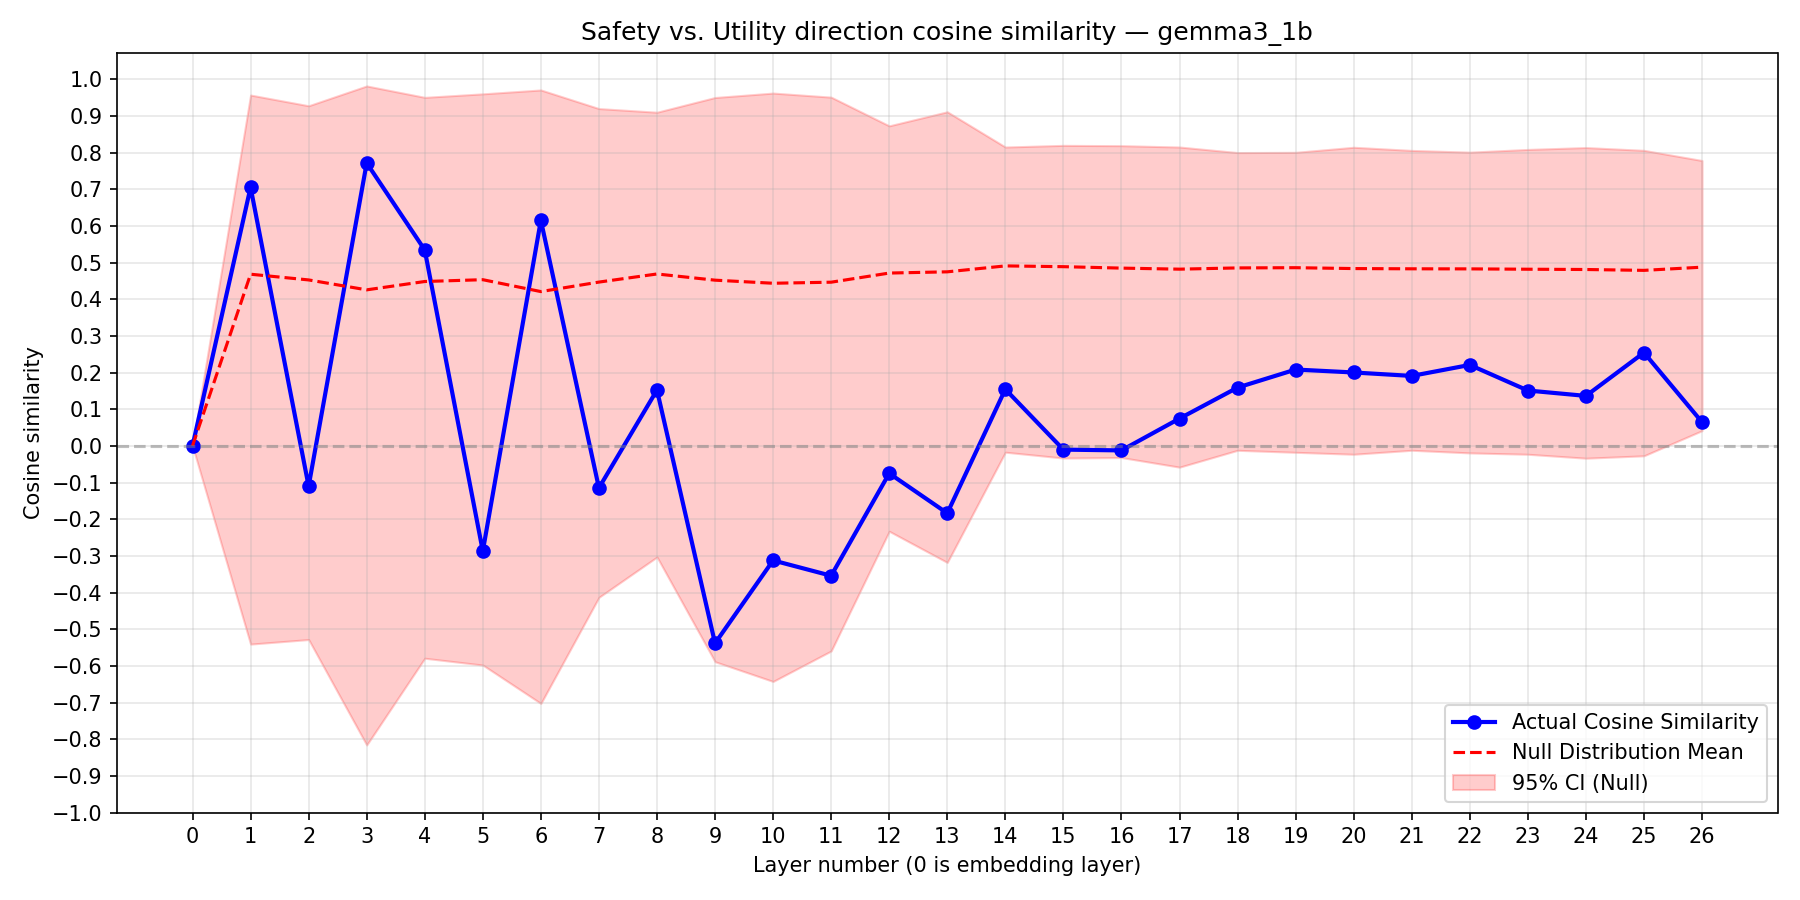
\includegraphics[width=0.95\linewidth]{../images/gemma3_1b_cosine_similarity.png}
    \caption{DoM cosine similarity per layer --- Gemma-3-1B-IT.}
    \label{fig:dom-gemma3-1b}
\end{figure}

\begin{figure}[h]
    \centering
    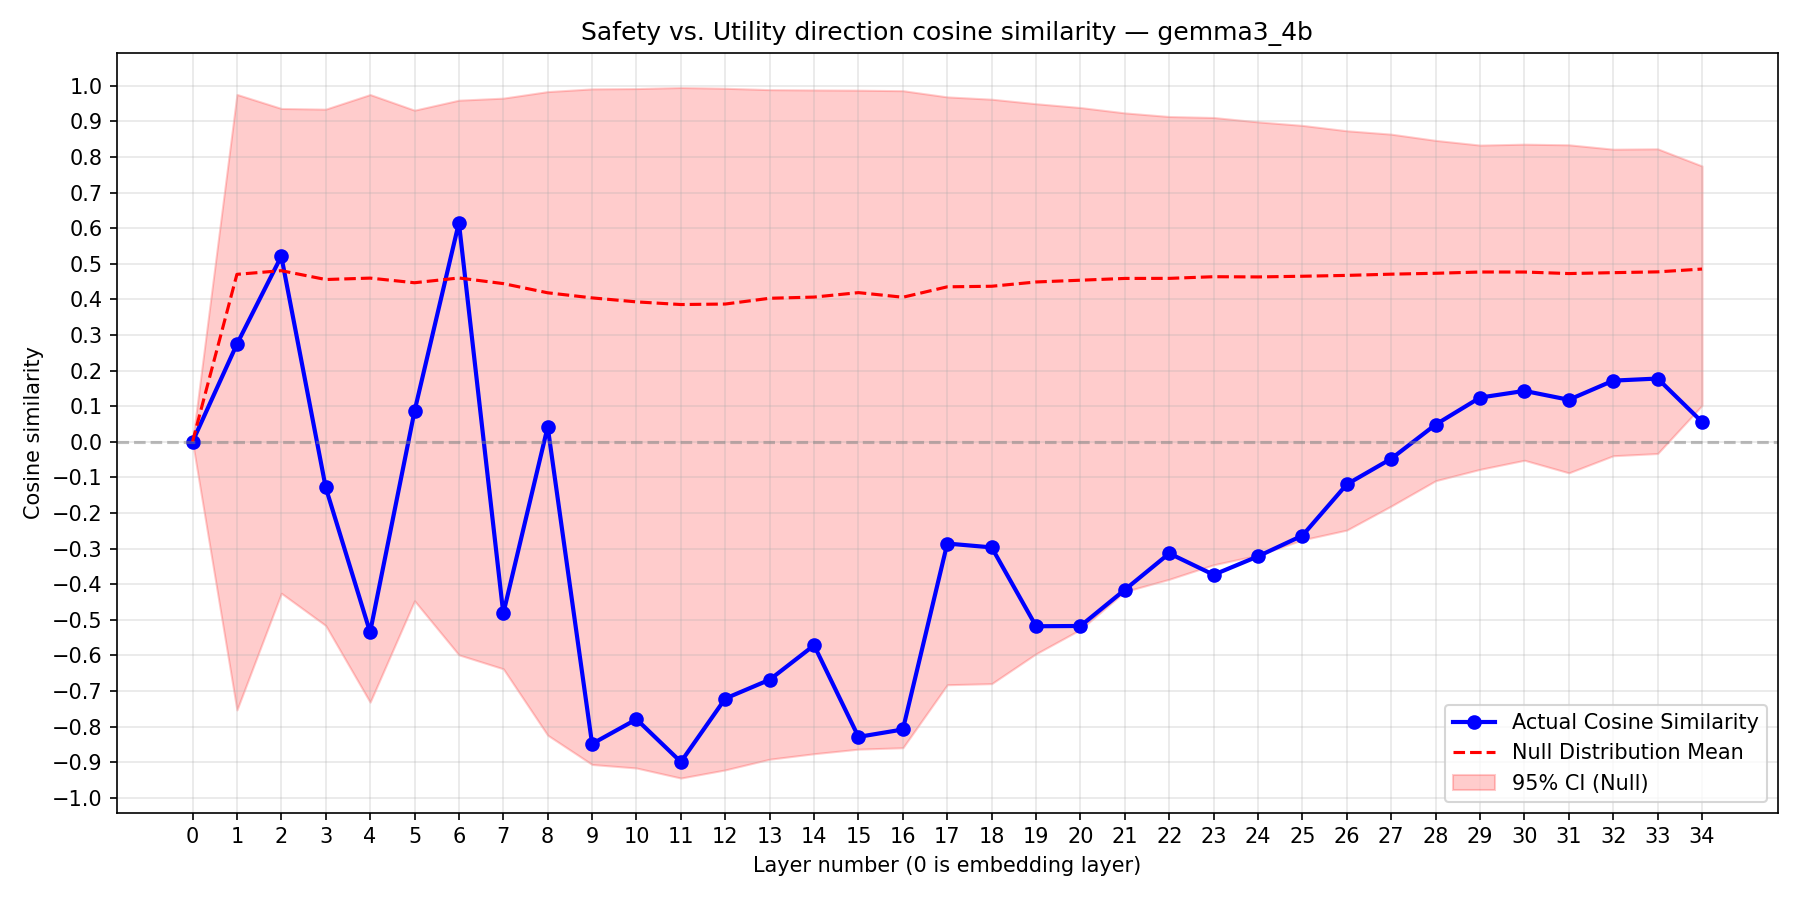
\includegraphics[width=0.95\linewidth]{../images/gemma3_4b_cosine_similarity.png}
    \caption{DoM cosine similarity per layer --- Gemma-3-4B-IT.}
    \label{fig:dom-gemma3-4b}
\end{figure}

\begin{figure}[h]
    \centering
    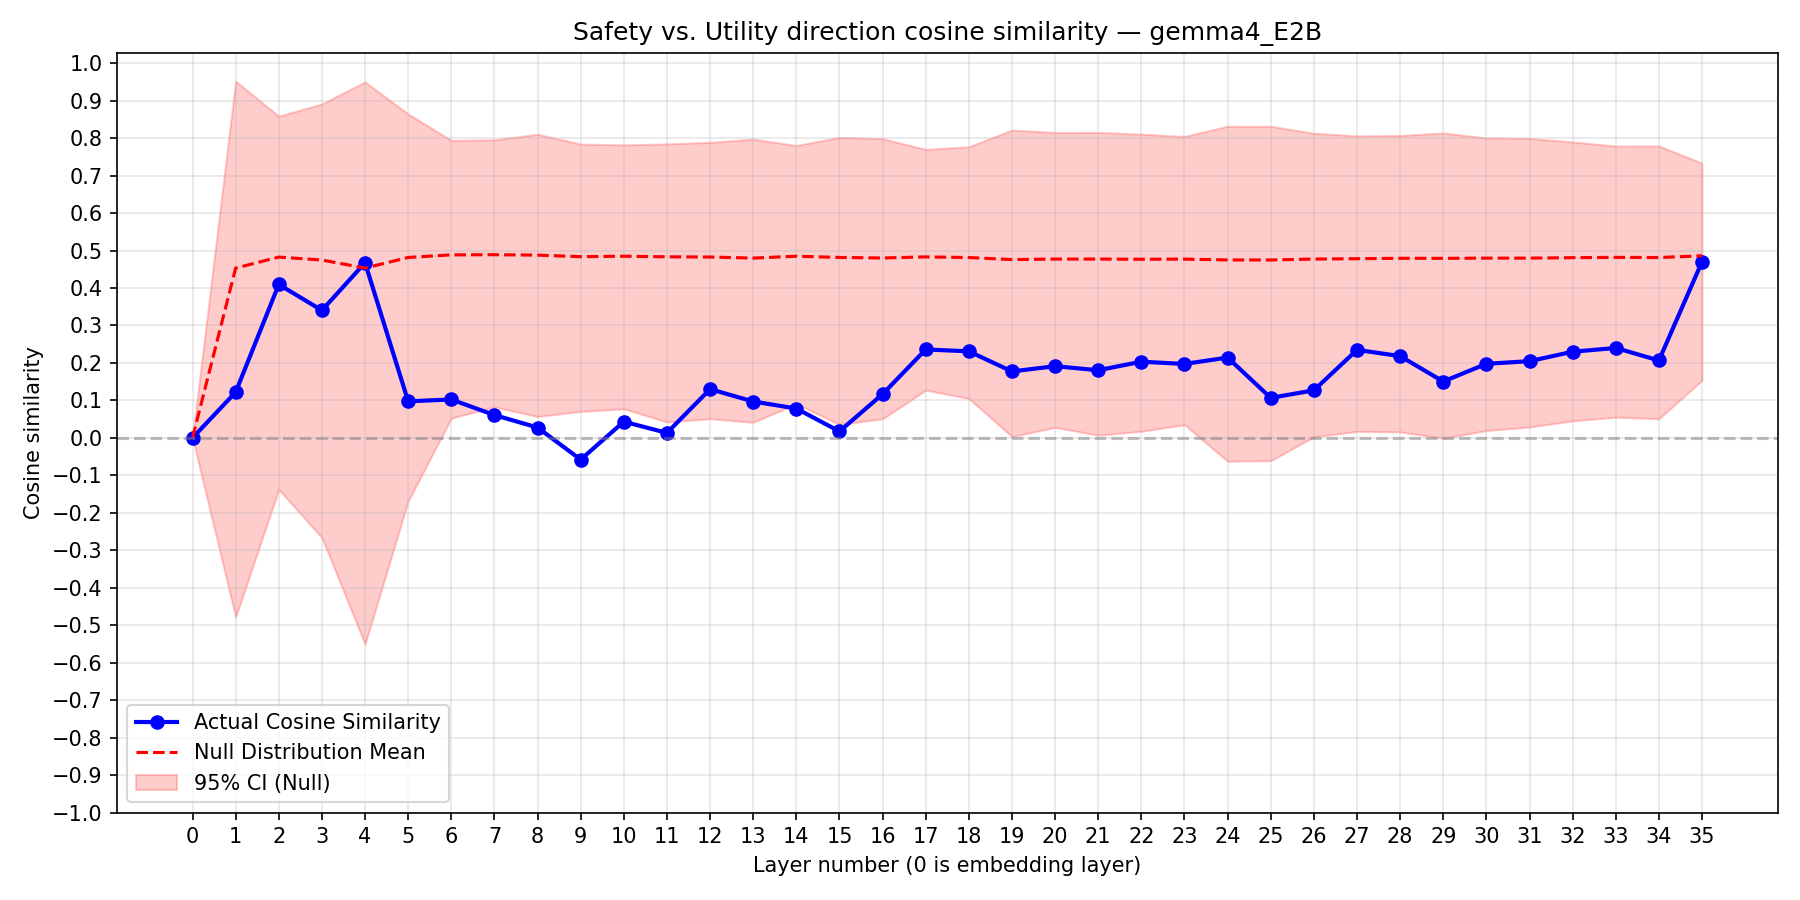
\includegraphics[width=0.95\linewidth]{../images/gemma4_E2B_cosine_similarity.png}
    \caption{DoM cosine similarity per layer --- Gemma-4-E2B-IT.}
    \label{fig:dom-gemma4-e2b}
\end{figure}

\begin{figure}[h]
    \centering
    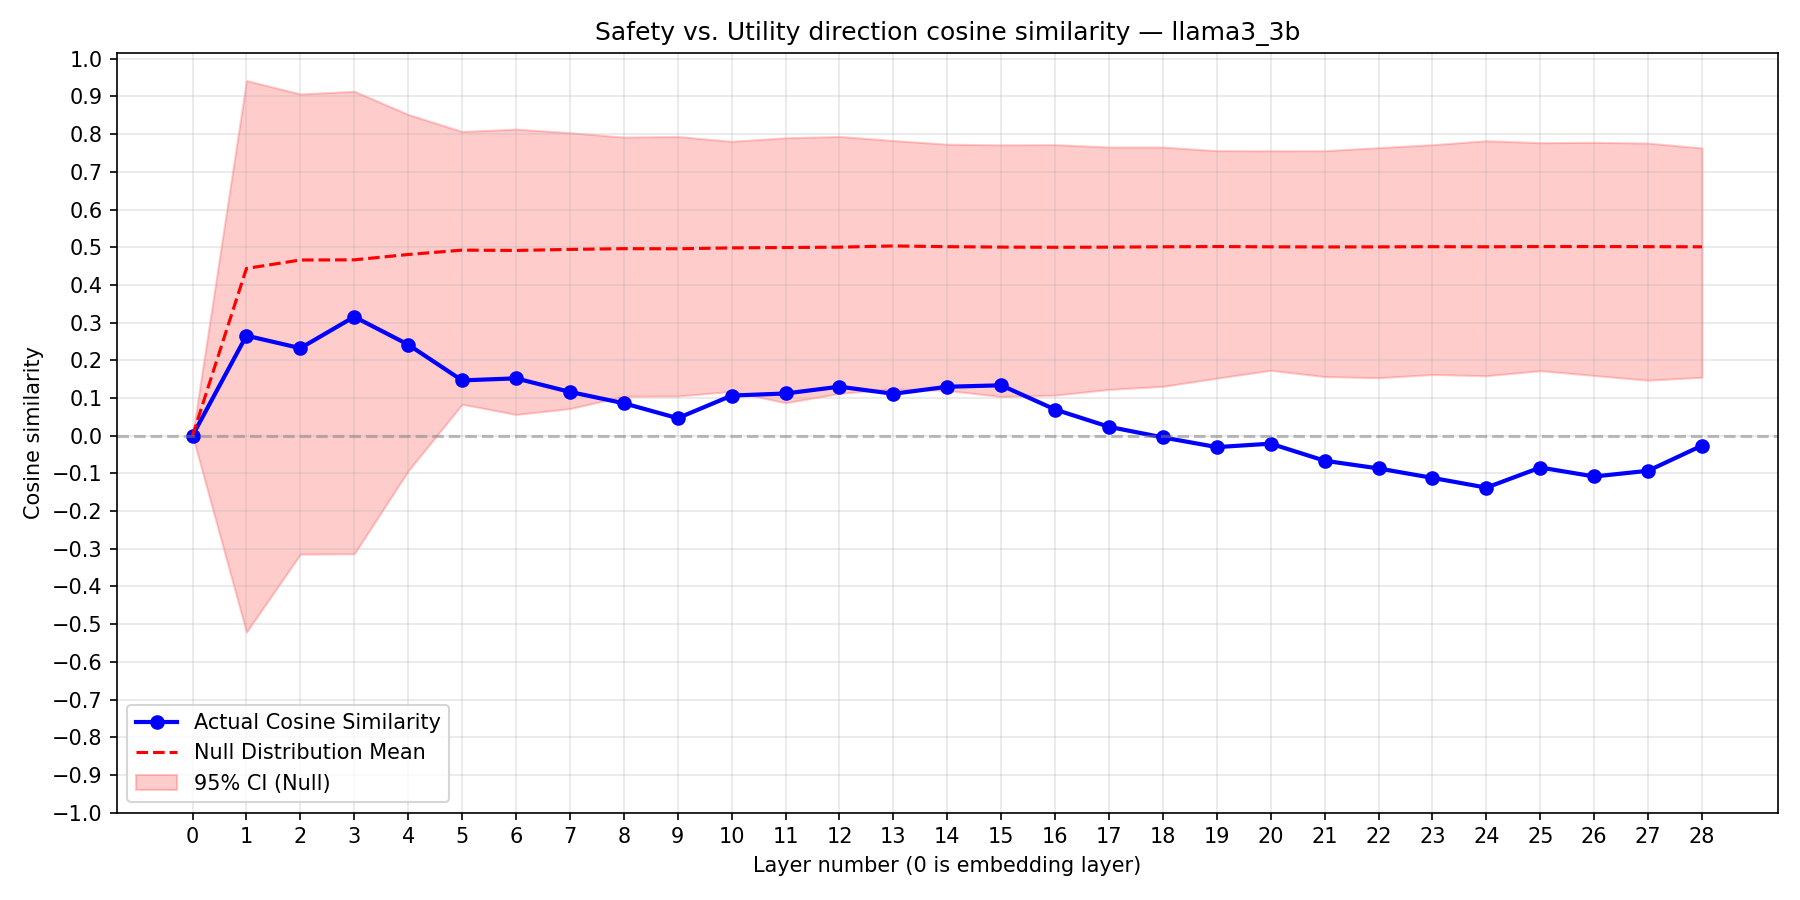
\includegraphics[width=0.95\linewidth]{../images/llama3_3b_cosine_similarity.png}
    \caption{DoM cosine similarity per layer --- Llama-3.2-3B-Instruct.}
    \label{fig:dom-llama3-3b}
\end{figure}

\begin{figure}[h]
    \centering
    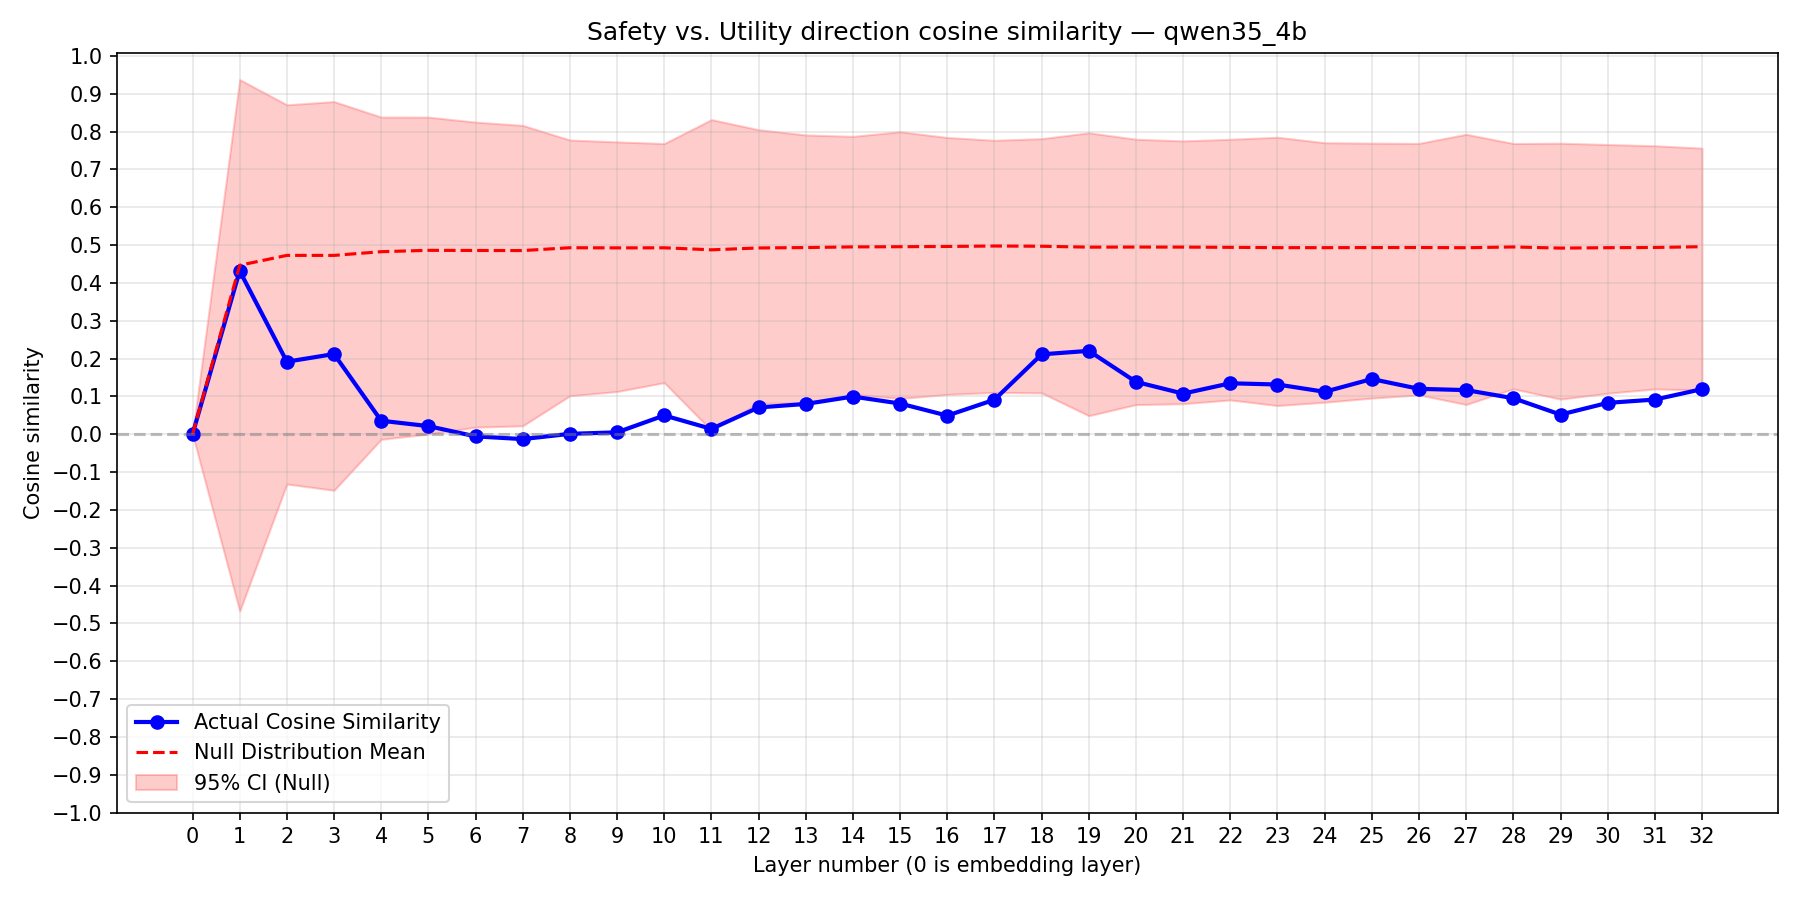
\includegraphics[width=0.95\linewidth]{../images/qwen35_4b_cosine_similarity.png}
    \caption{DoM cosine similarity per layer --- Qwen-3.5-4B.}
    \label{fig:dom-qwen35-4b}
\end{figure}

\subsection{ActSVD and Contrastive SVD subspace overlap}
\label{sec:figures-actsvd}

\begin{figure}[h]
    \centering
    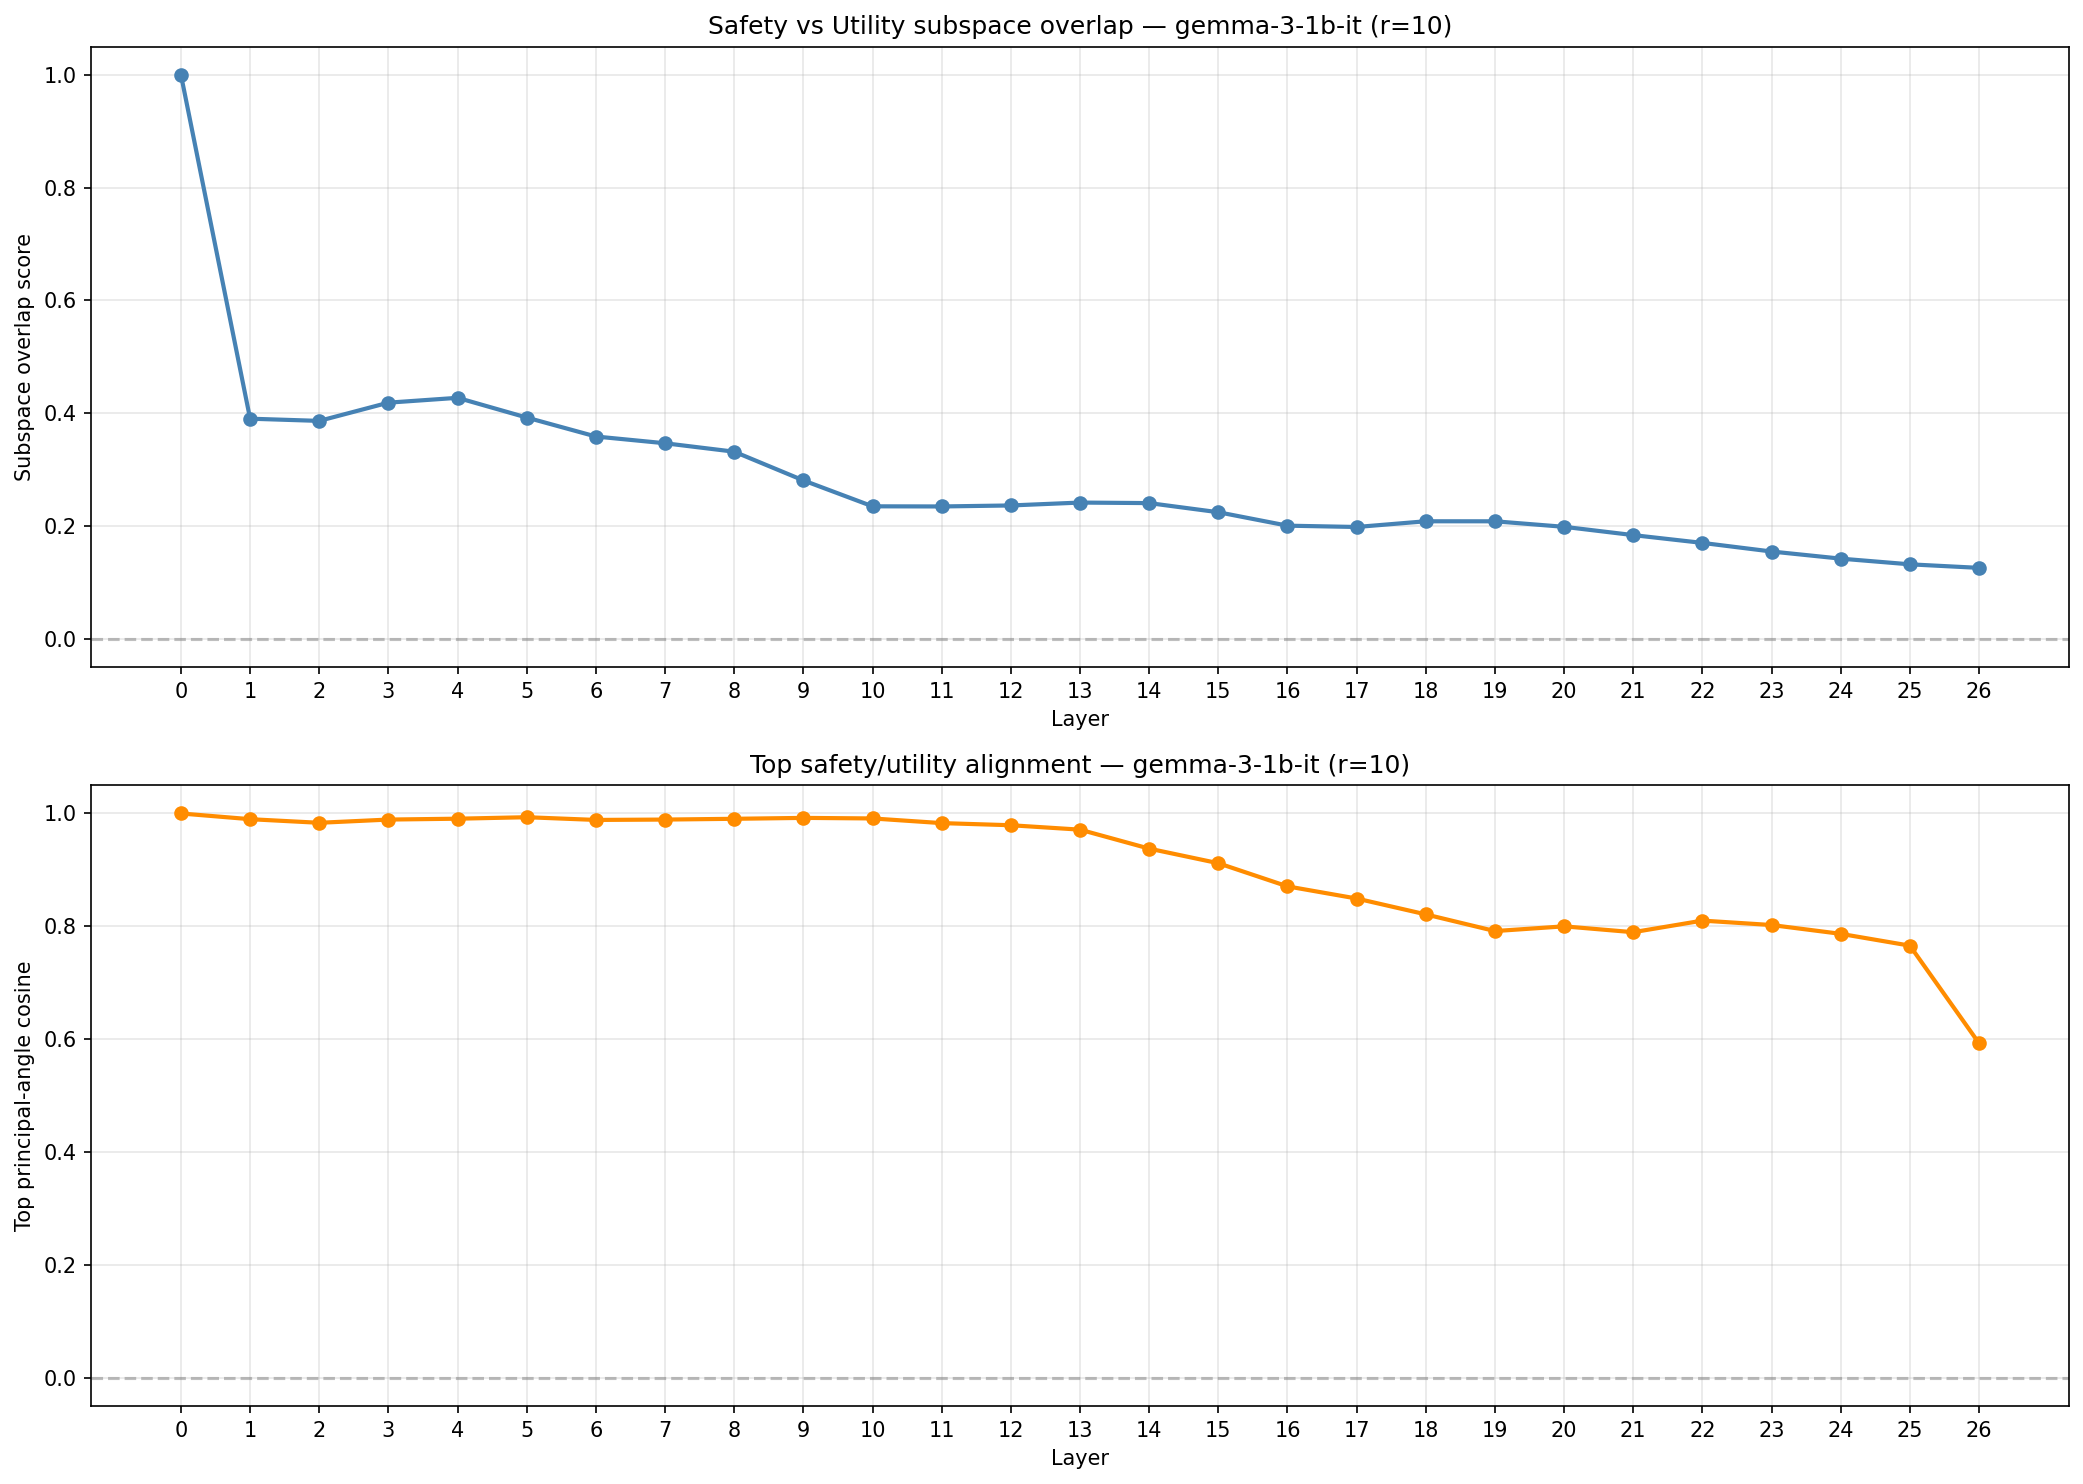
\includegraphics[width=0.95\linewidth]{../images/overlap_gemma-3-1b-it.png}
    \caption{ActSVD subspace overlap --- Gemma-3-1B-IT.}
    \label{fig:actsvd-gemma3-1b}
\end{figure}

\begin{figure}[h]
    \centering
    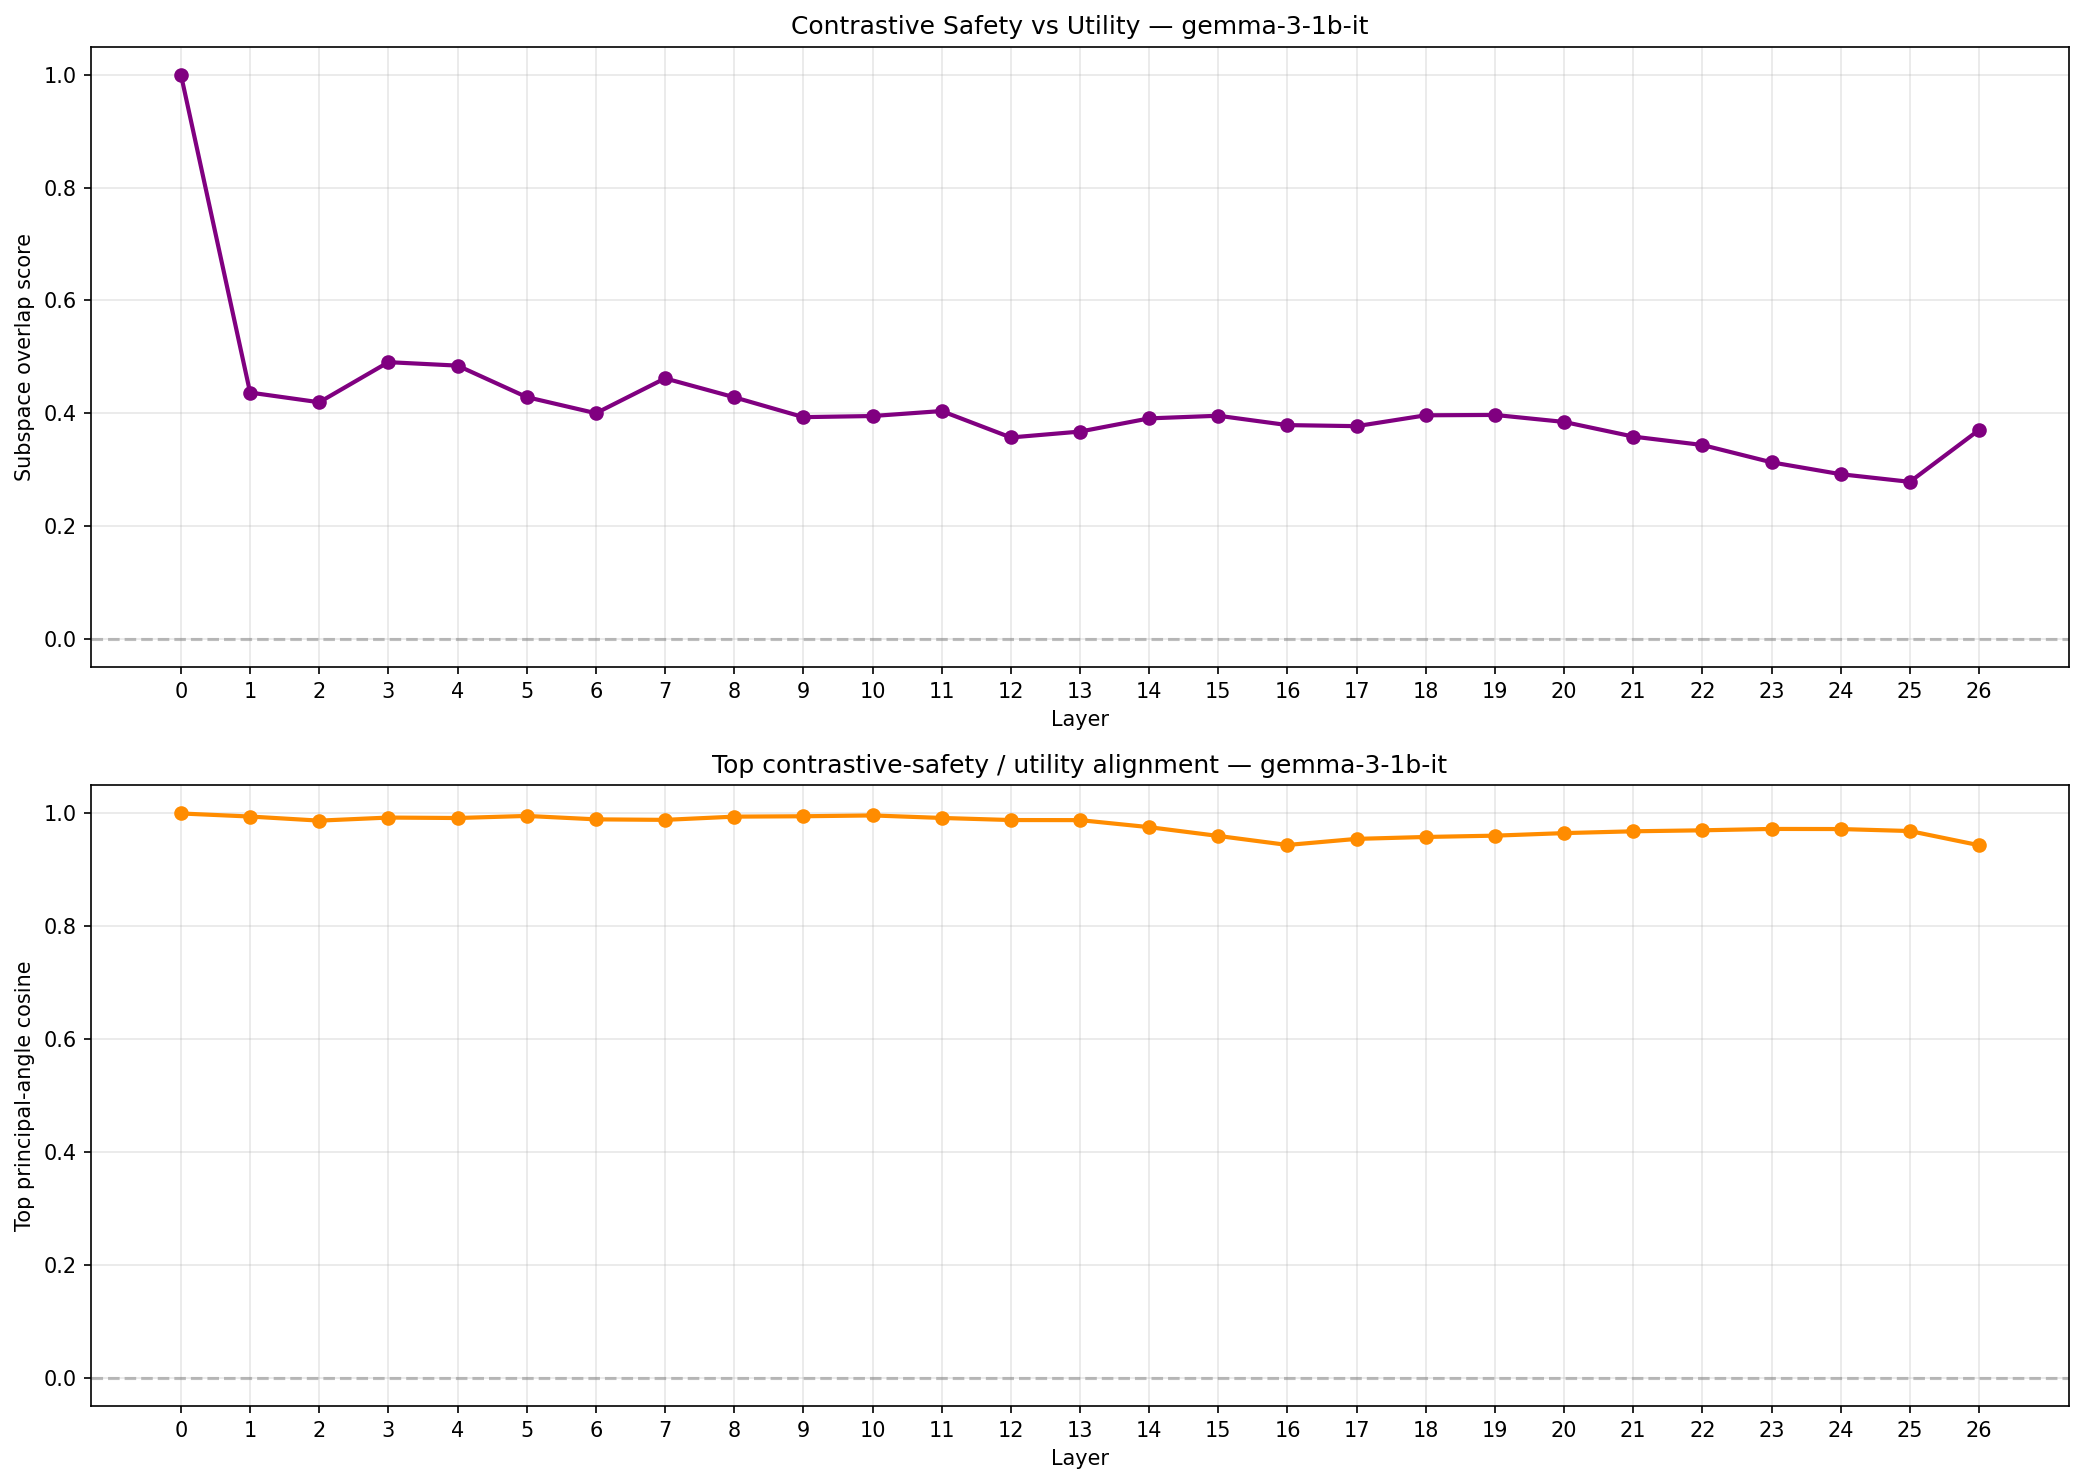
\includegraphics[width=0.95\linewidth]{../images/csvd_overlap_gemma-3-1b-it.png}
    \caption{Contrastive SVD subspace overlap --- Gemma-3-1B-IT.}
    \label{fig:csvd-gemma3-1b}
\end{figure}

\begin{figure}[h]
    \centering
    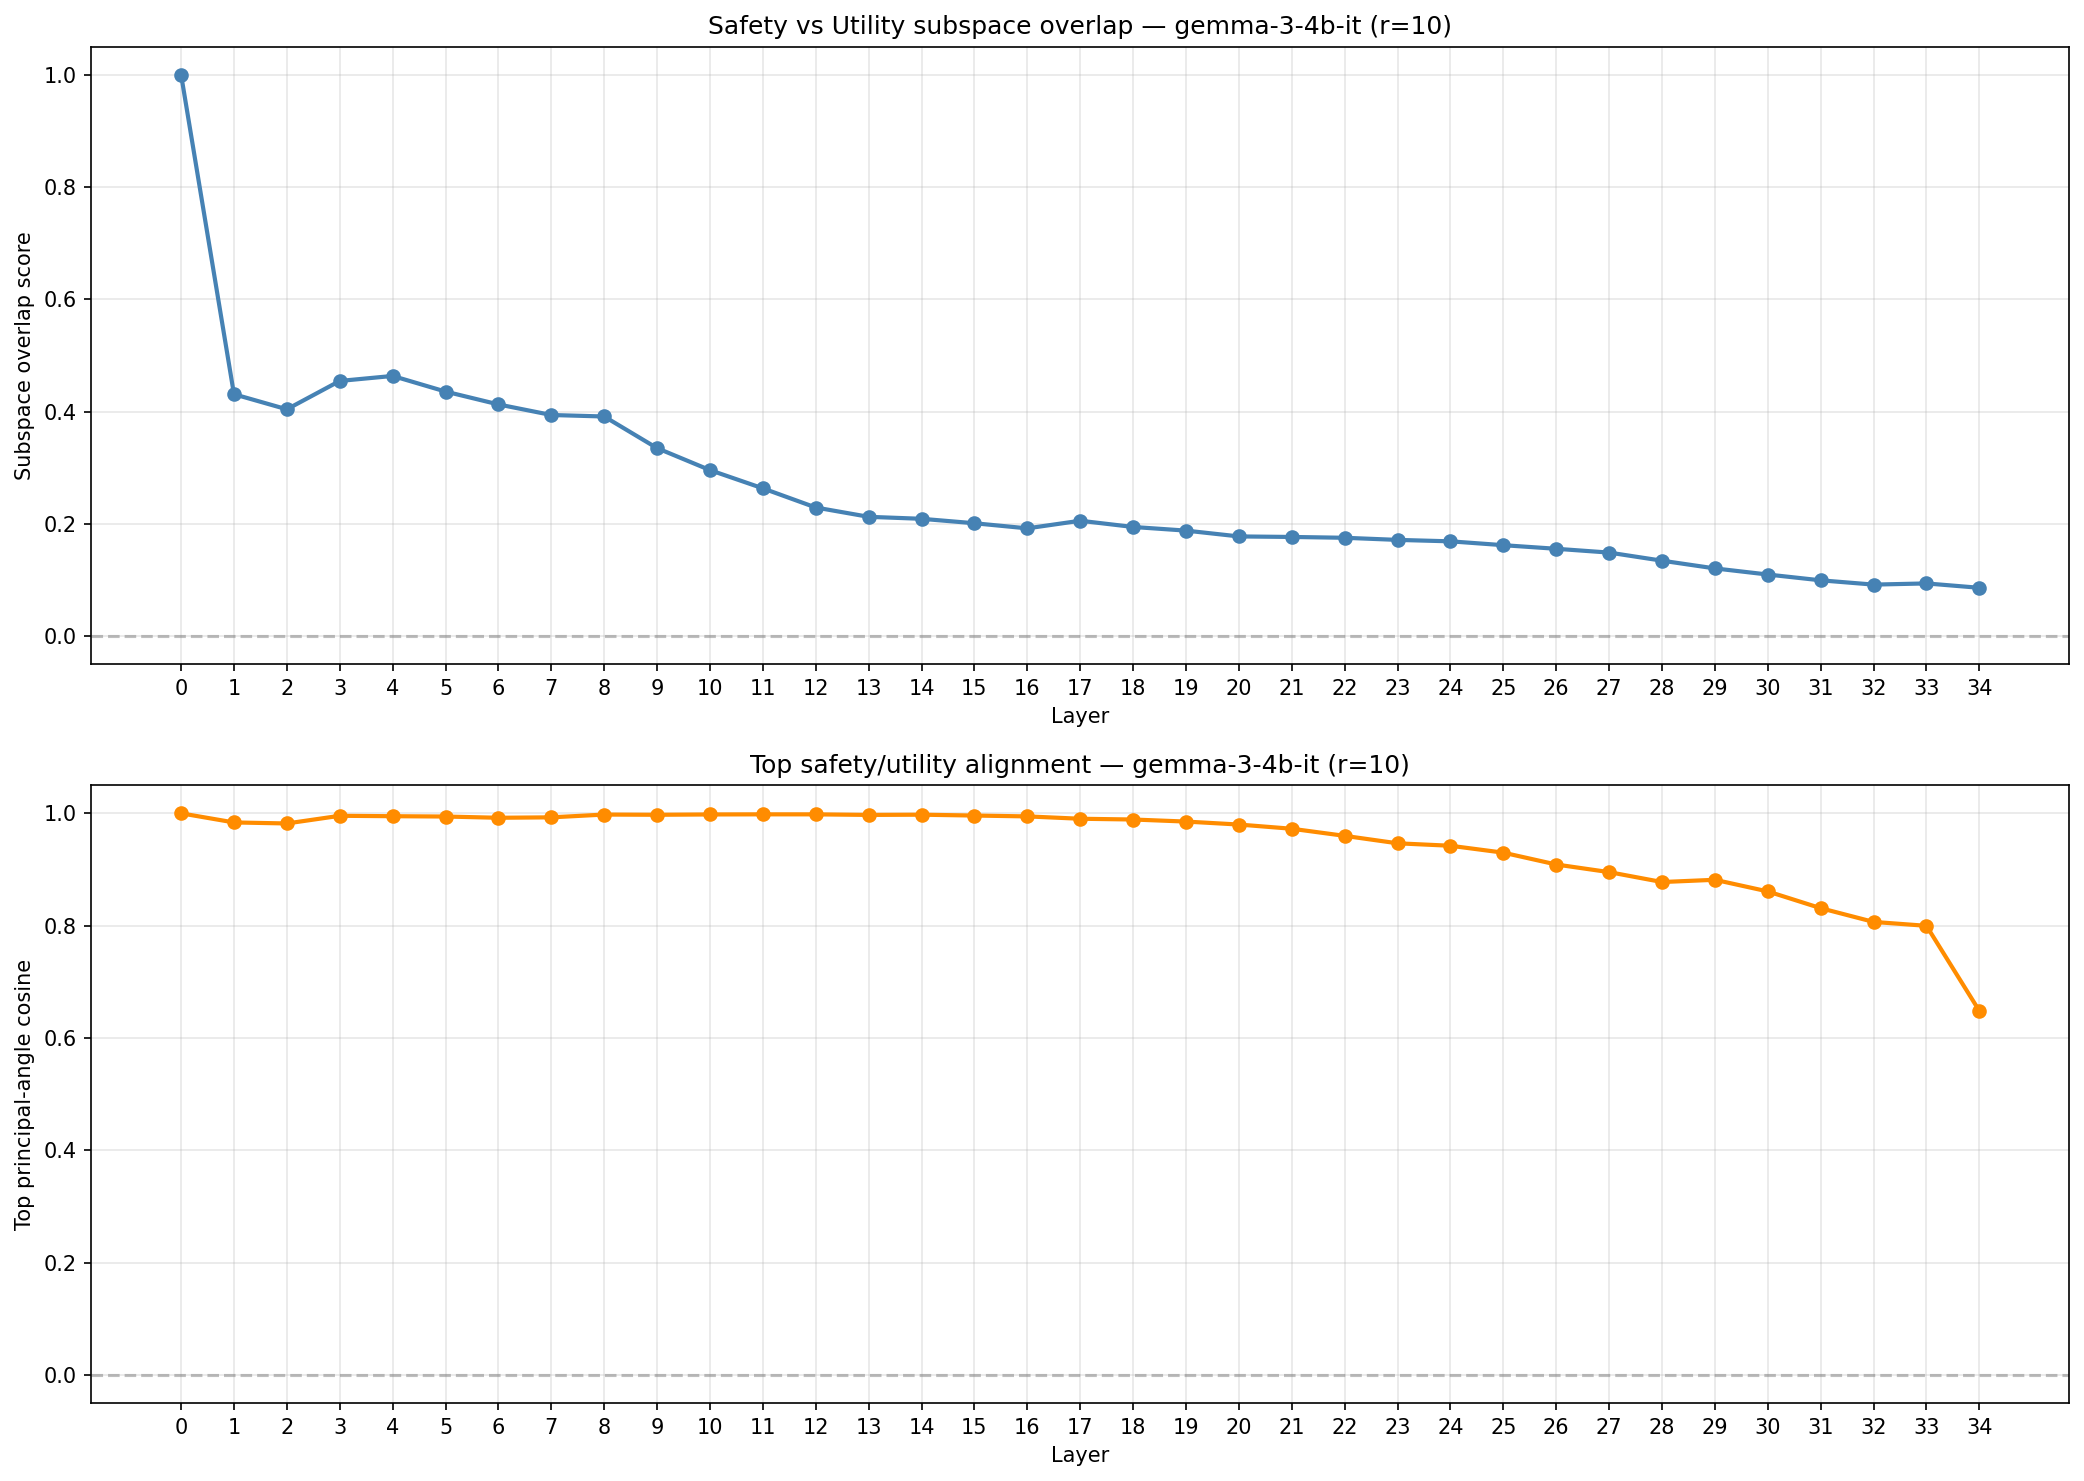
\includegraphics[width=0.95\linewidth]{../images/overlap_gemma-3-4b-it.png}
    \caption{ActSVD subspace overlap --- Gemma-3-4B-IT.}
    \label{fig:actsvd-gemma3-4b}
\end{figure}

\begin{figure}[h]
    \centering
    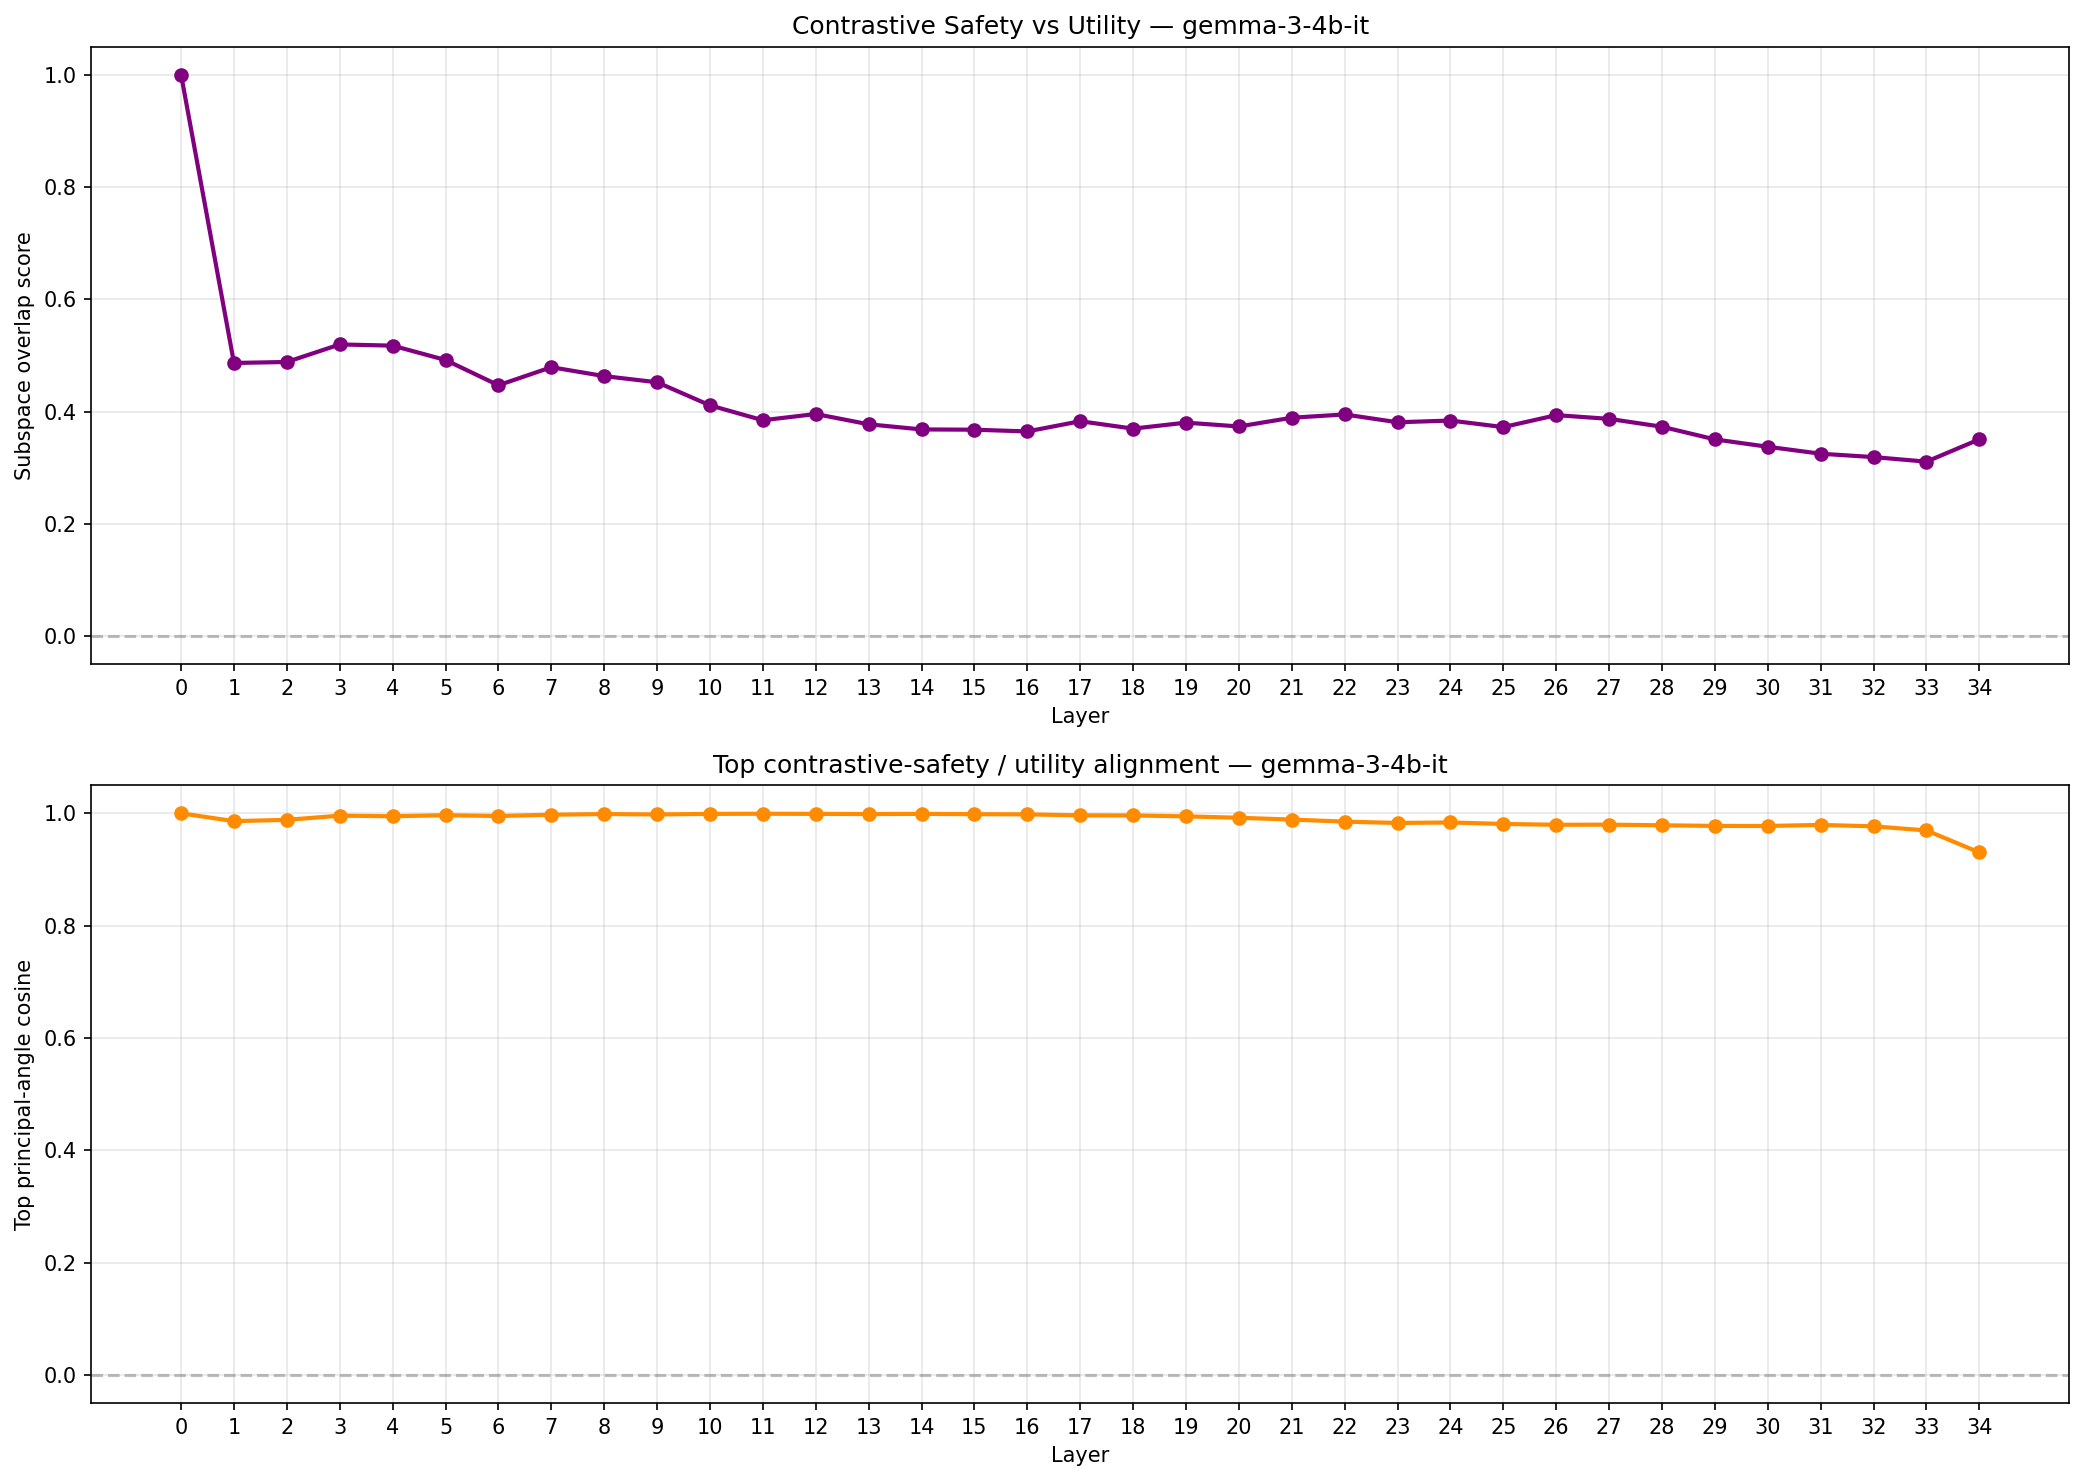
\includegraphics[width=0.95\linewidth]{../images/csvd_overlap_gemma-3-4b-it.png}
    \caption{Contrastive SVD subspace overlap --- Gemma-3-4B-IT.}
    \label{fig:csvd-gemma3-4b}
\end{figure}

\begin{figure}[h]
    \centering
    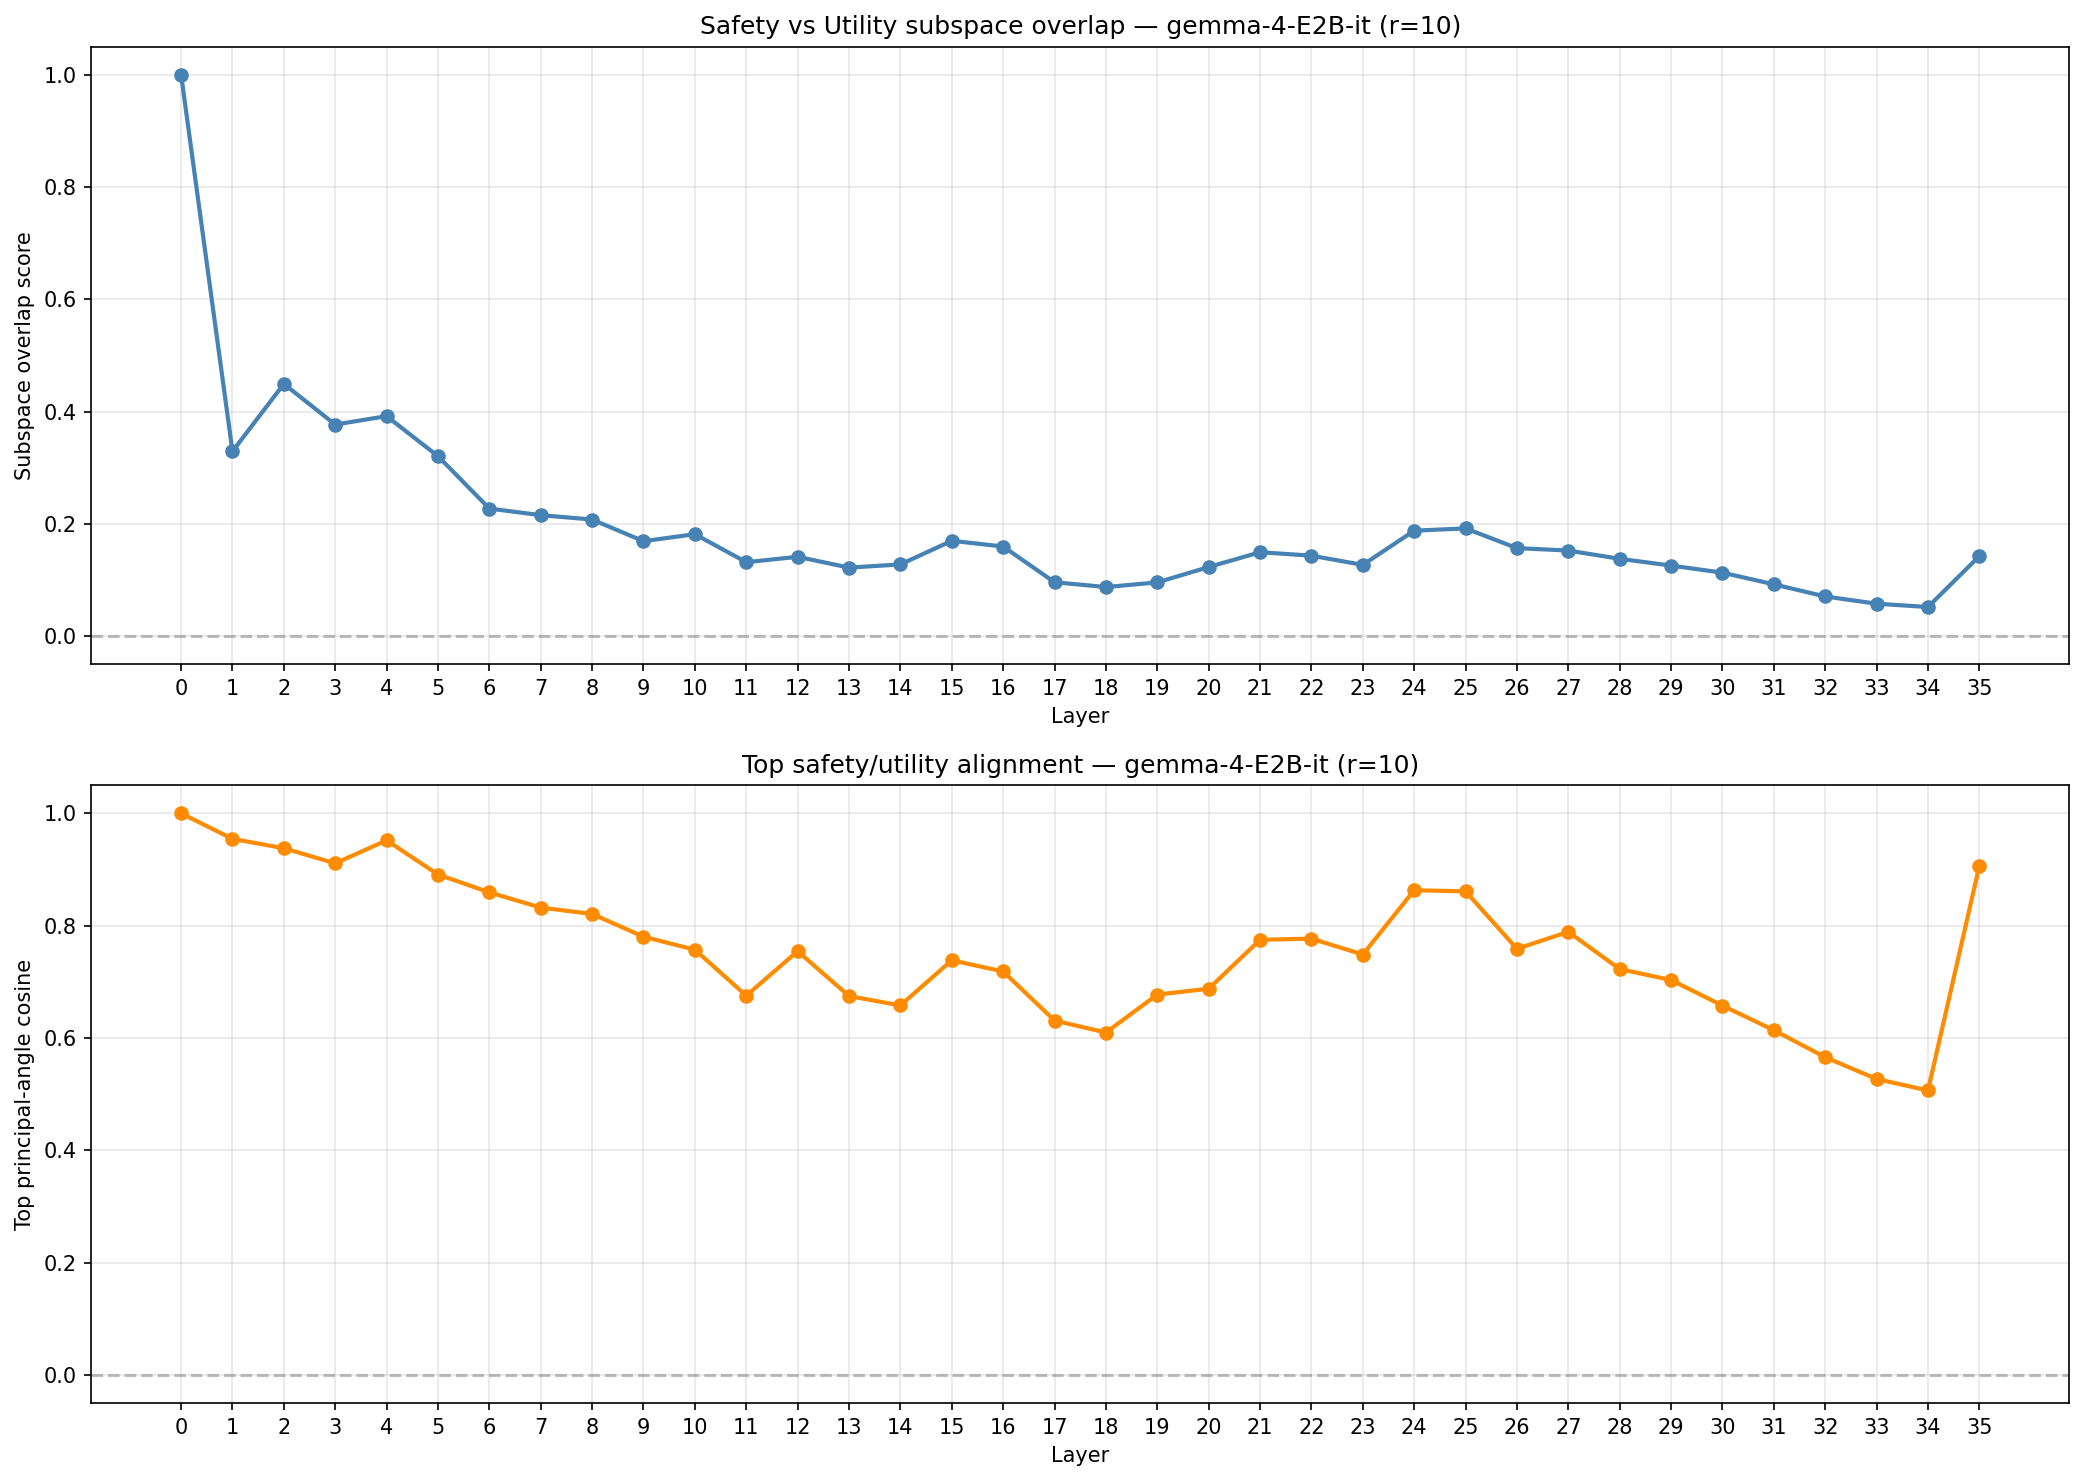
\includegraphics[width=0.95\linewidth]{../images/overlap_gemma-4-E2B-it.png}
    \caption{ActSVD subspace overlap --- Gemma-4-E2B-IT.}
    \label{fig:actsvd-gemma4-e2b}
\end{figure}

\begin{figure}[h]
    \centering
    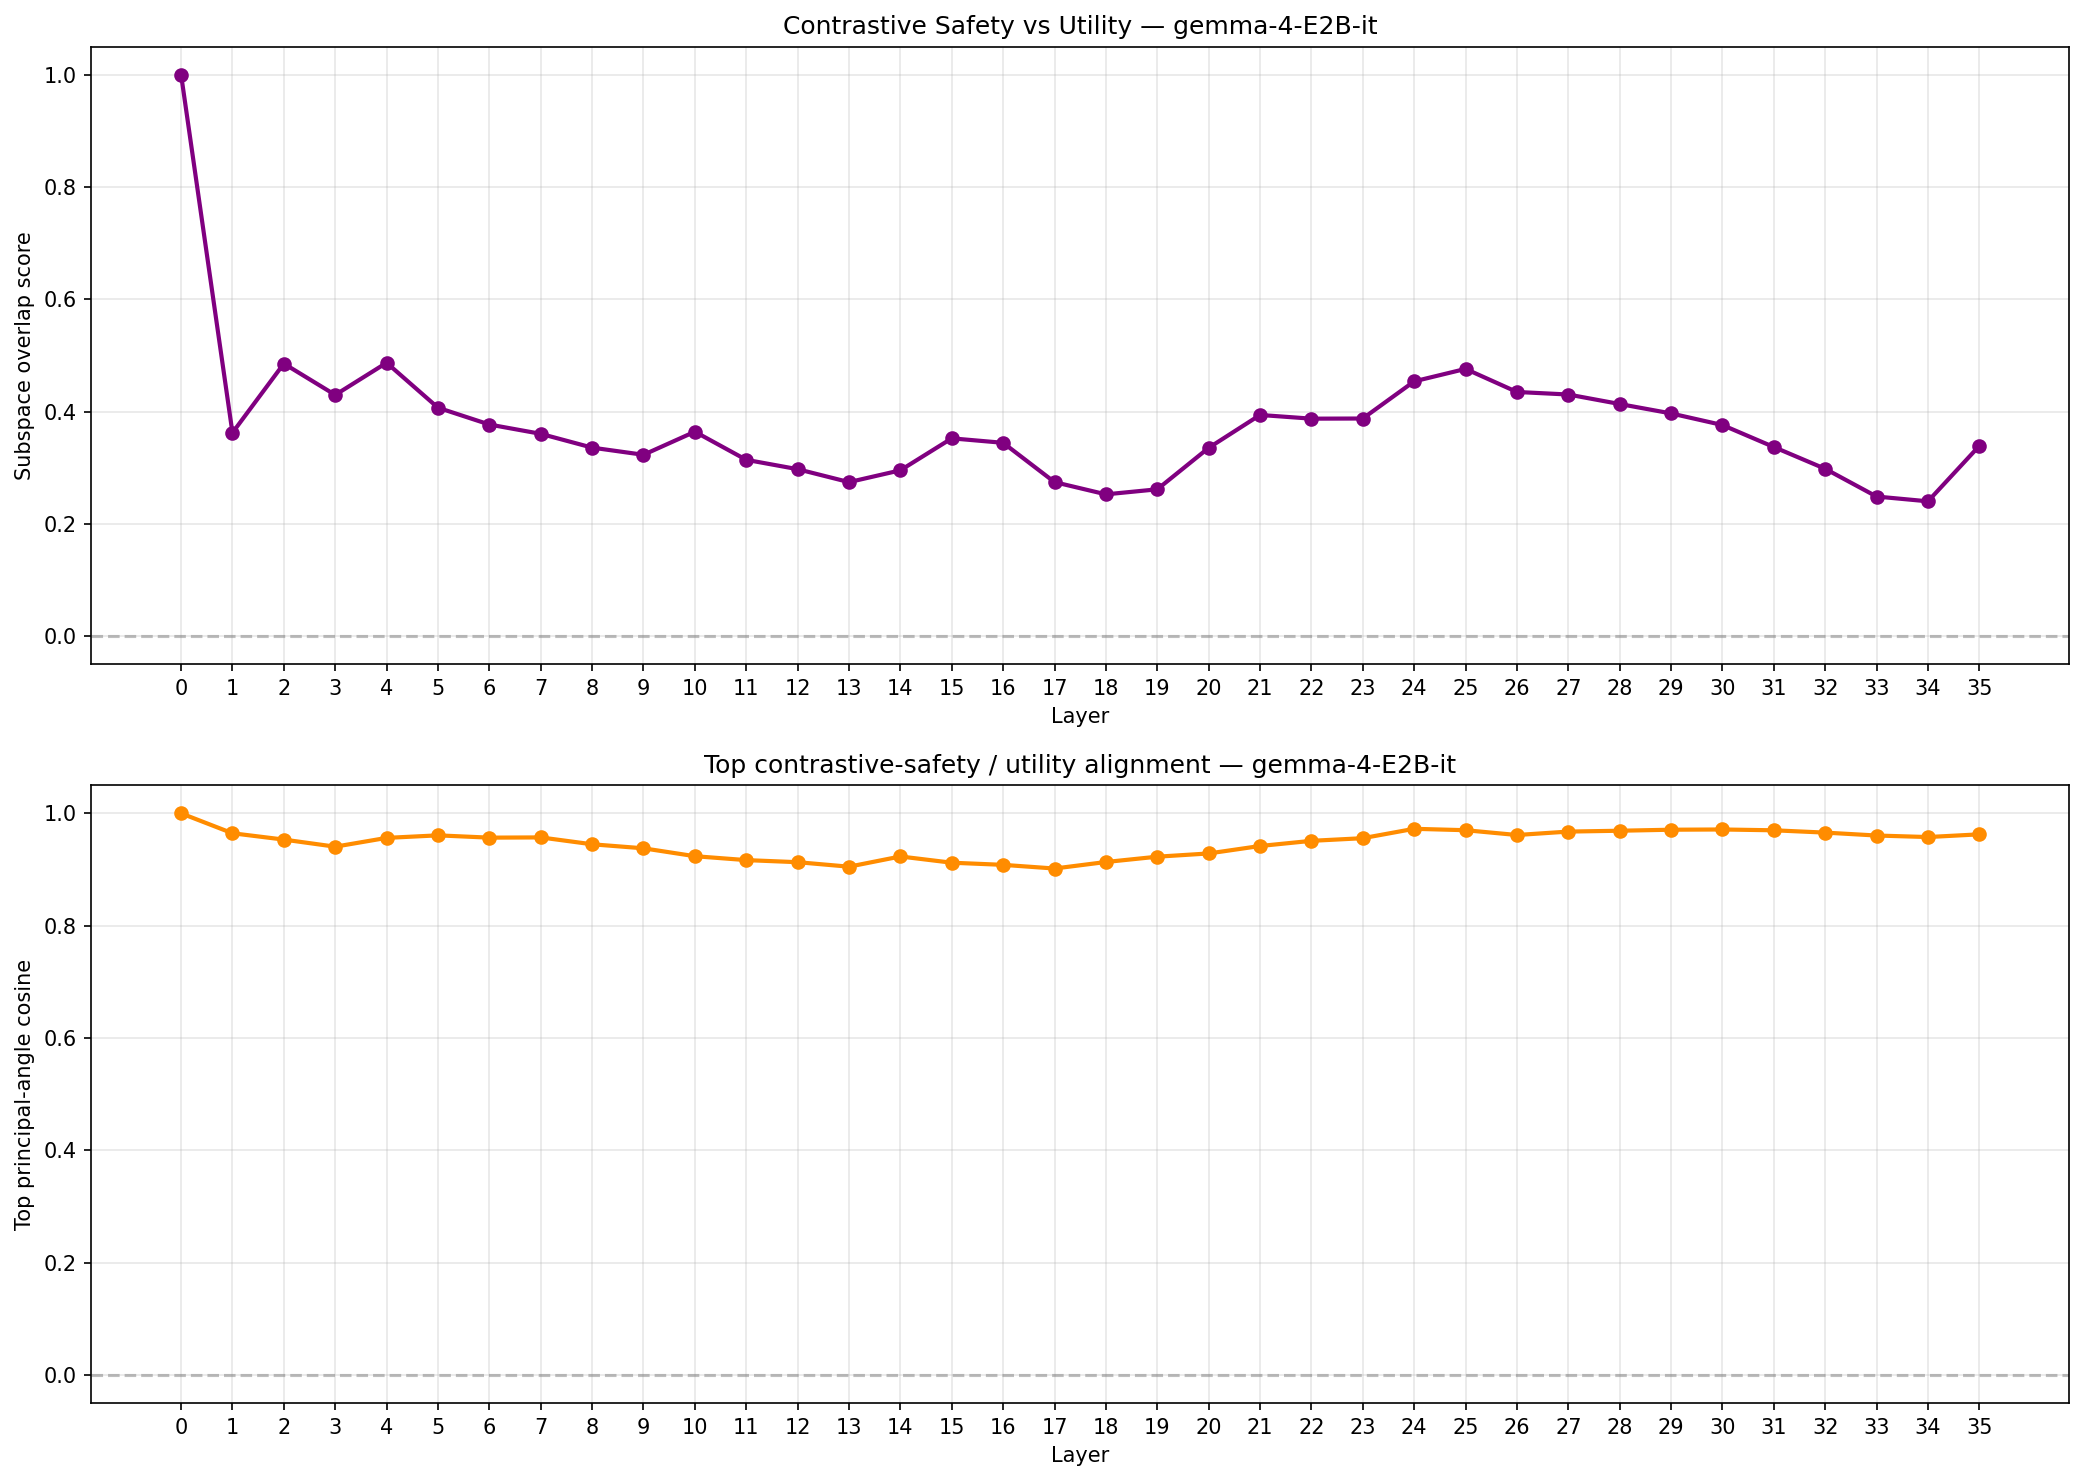
\includegraphics[width=0.95\linewidth]{../images/csvd_overlap_gemma-4-E2B-it.png}
    \caption{Contrastive SVD subspace overlap --- Gemma-4-E2B-IT.}
    \label{fig:csvd-gemma4-e2b}
\end{figure}

\begin{figure}[h]
    \centering
    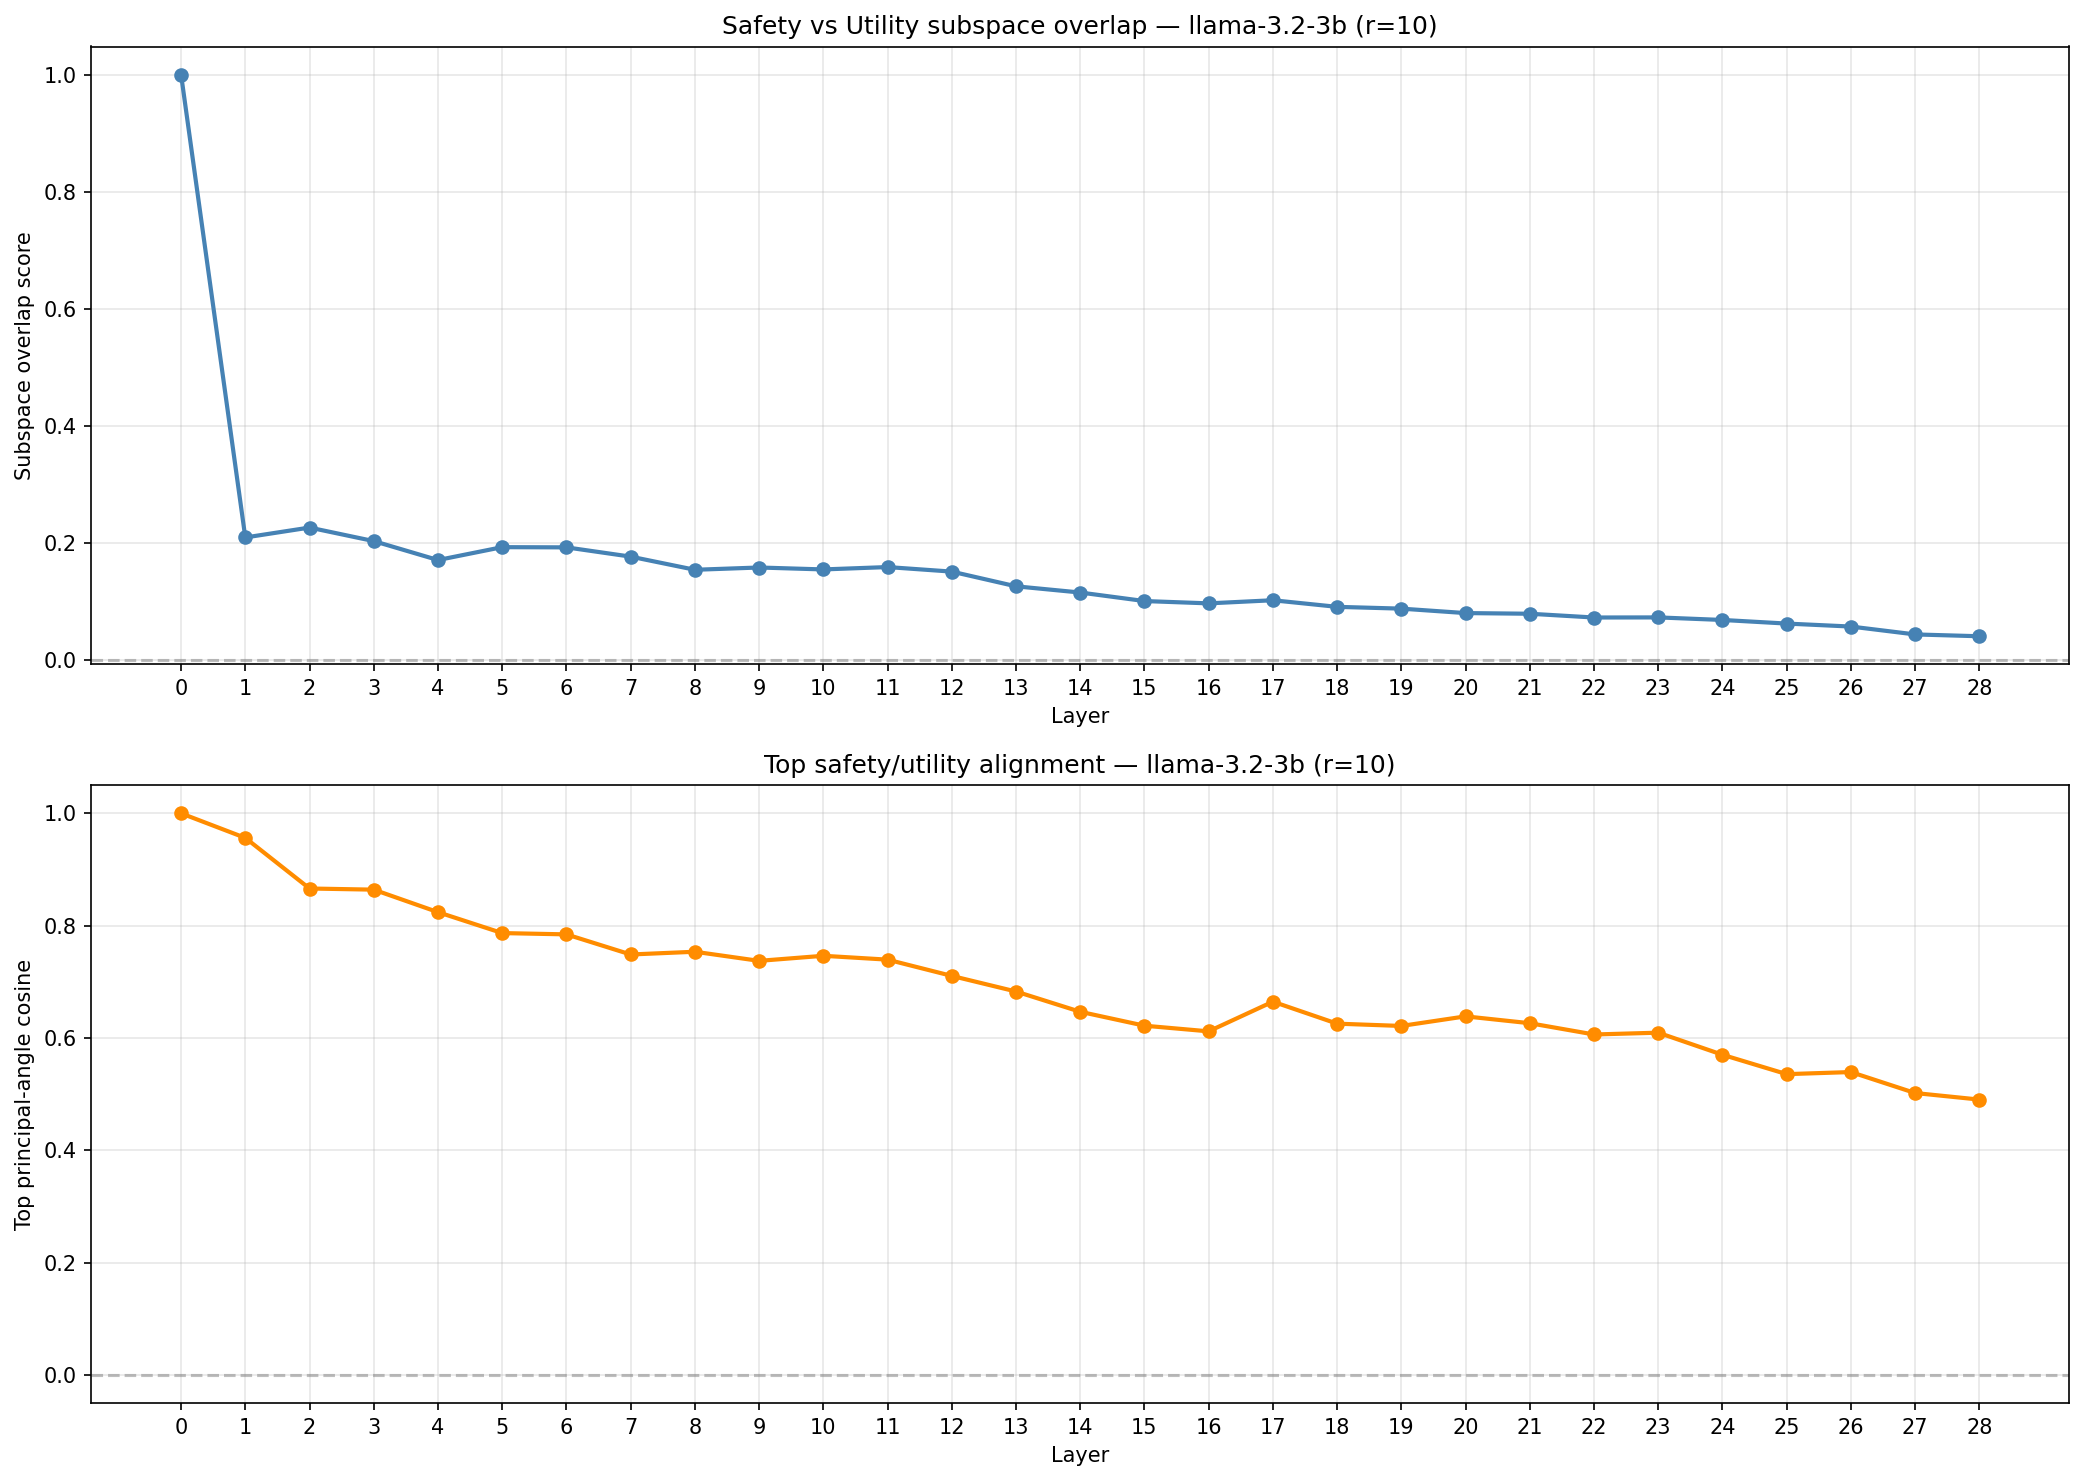
\includegraphics[width=0.95\linewidth]{../images/overlap_llama-3.2-3b.png}
    \caption{ActSVD subspace overlap --- Llama-3.2-3B-Instruct.}
    \label{fig:actsvd-llama3-3b}
\end{figure}

\begin{figure}[h]
    \centering
    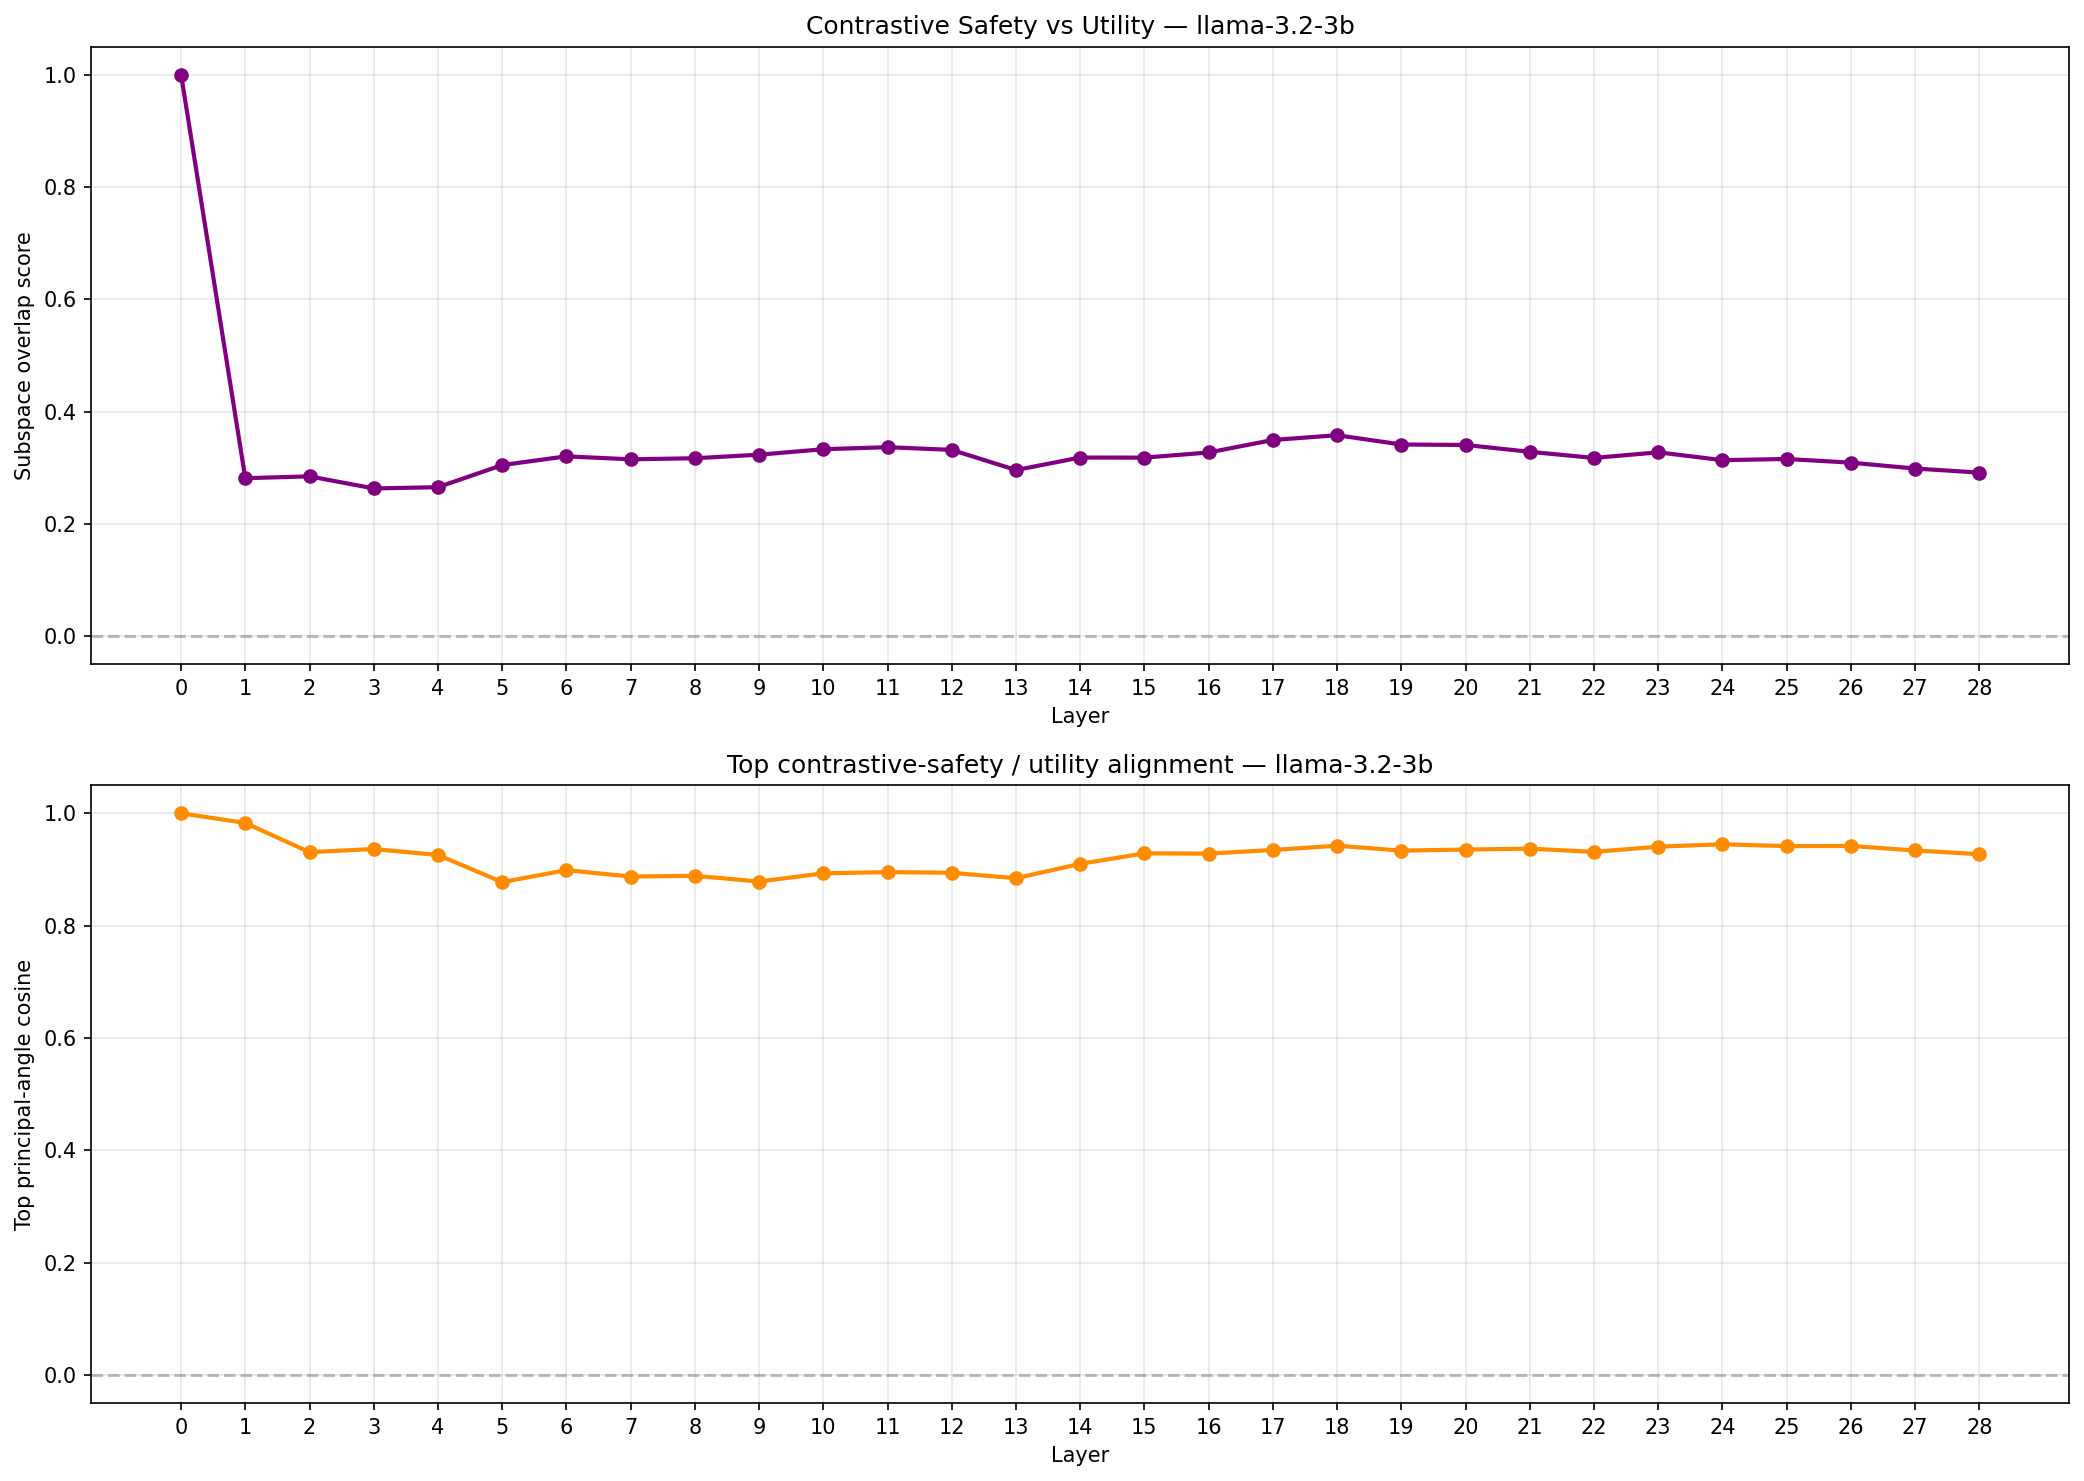
\includegraphics[width=0.95\linewidth]{../images/csvd_overlap_llama-3.2-3b.png}
    \caption{Contrastive SVD subspace overlap --- Llama-3.2-3B-Instruct.}
    \label{fig:csvd-llama3-3b}
\end{figure}

\begin{figure}[h]
    \centering
    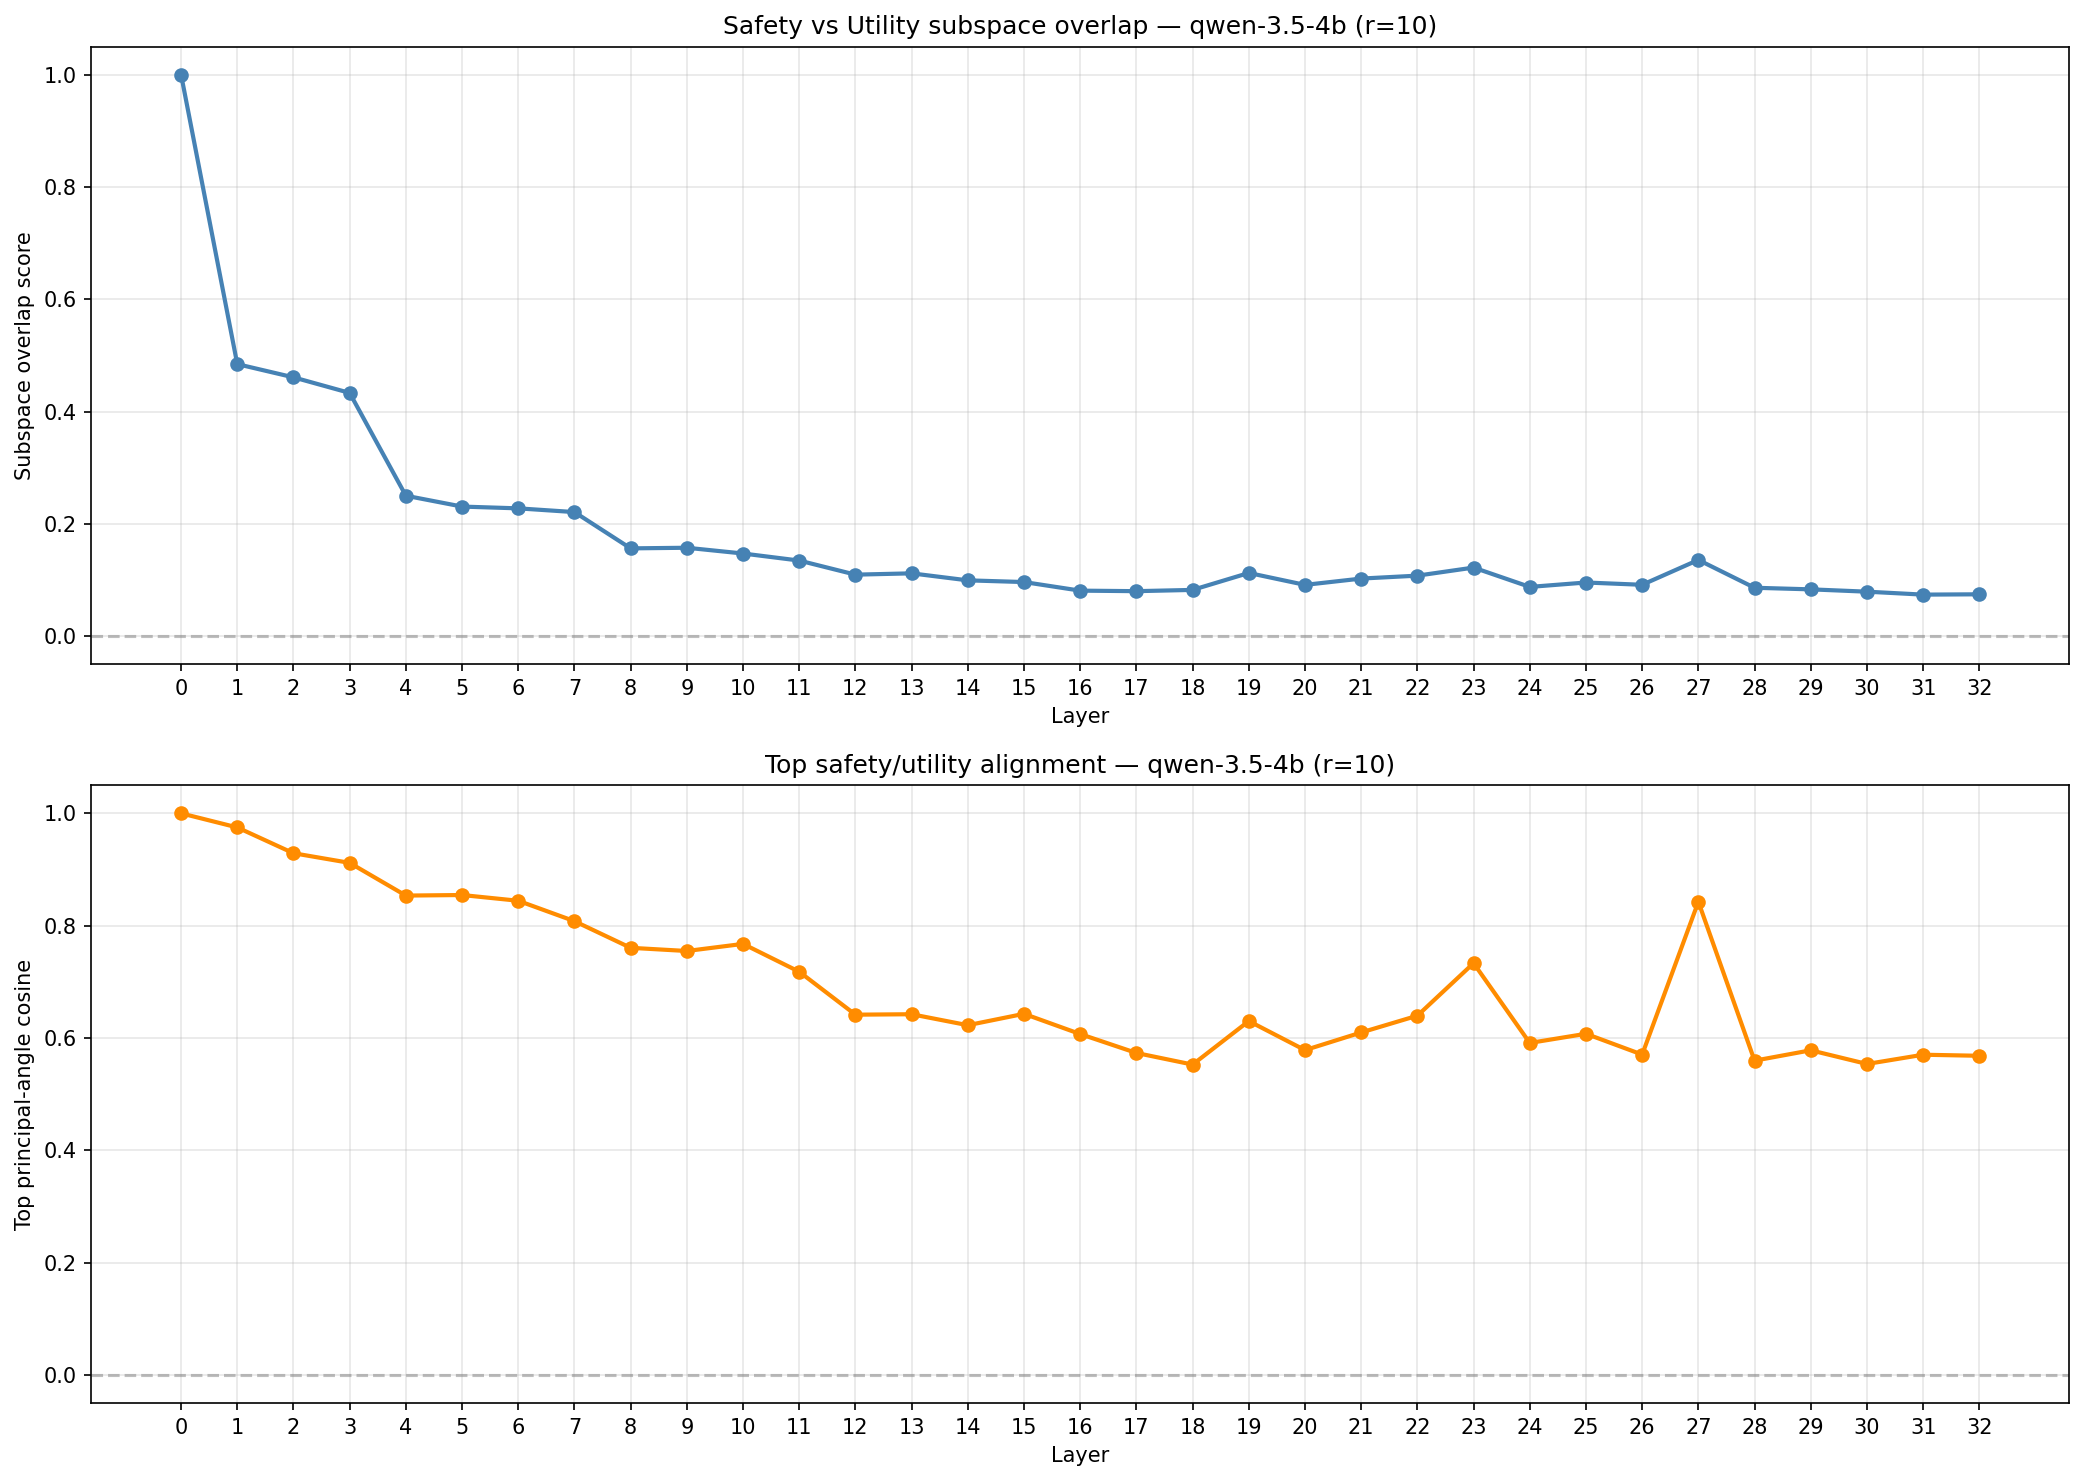
\includegraphics[width=0.95\linewidth]{../images/overlap_qwen-3.5-4b.png}
    \caption{ActSVD subspace overlap --- Qwen-3.5-4B.}
    \label{fig:actsvd-qwen35-4b}
\end{figure}

\begin{figure}[h]
    \centering
    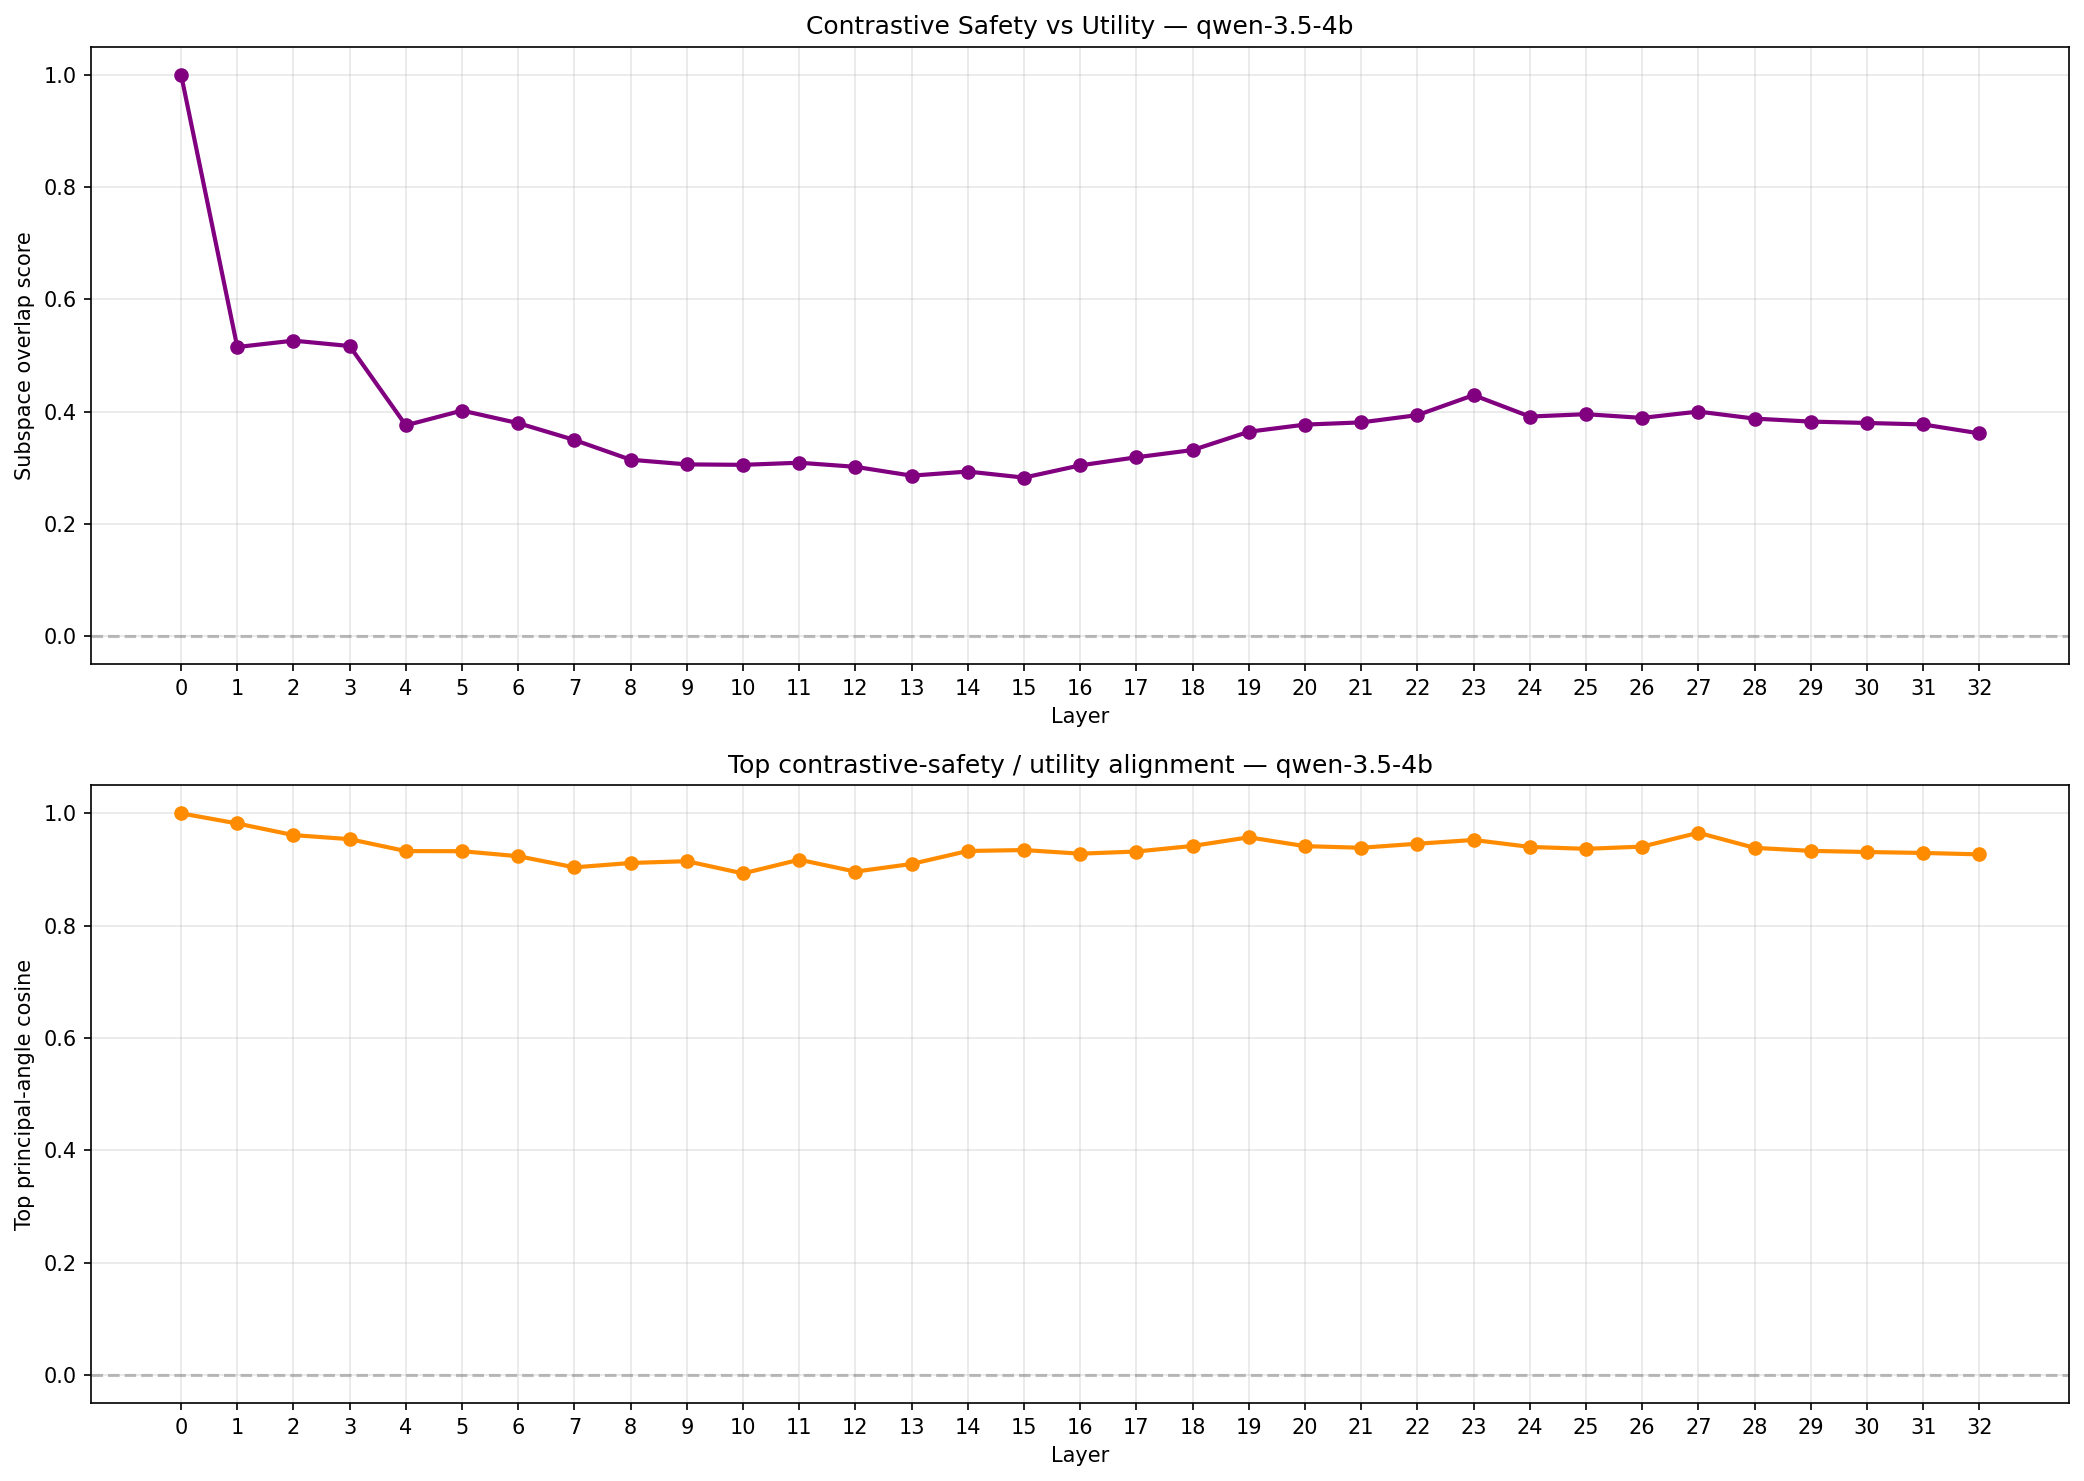
\includegraphics[width=0.95\linewidth]{../images/csvd_overlap_qwen-3.5-4b.png}
    \caption{Contrastive SVD subspace overlap --- Qwen-3.5-4B.}
    \label{fig:csvd-qwen35-4b}
\end{figure}
